\documentclass[aspectratio=169]{beamer}

% --- Configuración de Idioma y Codificación ---
\usepackage[utf8]{inputenc}
\usepackage[spanish, es-tabla]{babel}

% --- Matemáticas y Fuentes ---
\usepackage{amsmath}
\usepackage{amsfonts}
\usepackage{amssymb}
% ELIMINADO: \usepackage{mathds} (Causaba el error y no se usa en el cuerpo)

% --- Gráficos y TikZ ---
\usepackage{tikz}
\usepackage{tikz-3dplot}
\usepackage{pgfplots}
\usepackage{graphicx}
\usepackage{booktabs}
\usepackage{caption}
\usepackage{multimedia}
\usepackage{animate}
\usepackage{xcolor}
\usepackage{hyperref}
\usepackage{fontawesome}
% Configuración de TikZ y PGFPlots
\pgfplotsset{compat=1.18}
\usetikzlibrary{positioning, shapes.geometric, arrows.meta, calc, backgrounds, fit, shadows, patterns, babel}

% --- Tema de Beamer ---
\usetheme{Madrid}
\usecolortheme{dolphin}
\setbeamertemplate{navigation symbols}{}
% --- Título ---
\title[Reconocimiento de Patrones]{Trabajo: Técnicas de Reconocimiento de Patrones}
\subtitle{Detección de objetos en imágenes térmicas con YOLOv5}
\author{J. Bengoa \and B. Barañski \and S. Izquierdo }
\date{\today}

\begin{document}
	
	% Solución para conflictos de caracteres en babel-spanish dentro de TikZ
	\shorthandoff{<}
	\shorthandoff{>}
	
	% --- Slide 1: Título ---
	\begin{frame}
		\titlepage
	\end{frame}
	
	% --- Slide 2: Índice ---
	\begin{frame}{Índice}
		\tableofcontents
	\end{frame}
	
	% --- Sección 1: Introducción ---
	\section{Introducción}
	\begin{frame}{Índice}
		\tableofcontents[currentsection] 
	\end{frame}
	\begin{frame}{Introducción a la termografía (TIR)}
		% PARTE SUPERIOR: Contexto y Desafíos
		\textbf{Contexto:}
		\begin{itemize}
			\item Visión artificial crítica en seguridad y conducción autónoma.
			\item Imágenes RGB fallan con mala iluminación (niebla, noche).
			\item \textbf{Solución:} Termografía infrarroja (TIR) $\rightarrow$ detecta radiación térmica.
		\end{itemize}
		
		\vspace{0.2cm} % Espacio pequeño entre secciones
		
		\textbf{Desafíos en TIR:}
		\begin{itemize}
			\item Baja resolución (sensores caros), falta de color (monocanal).
			\item Texturas difusas y efecto halo.
		\end{itemize}
		
		\vfill % Empuja el objetivo al fondo
		
		% PARTE INFERIOR: Objetivo (Ancho completo o ajustado)
		\begin{columns}
			\column{0.9\textwidth} % Un poco menos de 1 para que no pegue a los bordes
			\begin{block}{Objetivo}
				Validar la arquitectura \textbf{YOLOv5} sobre el dataset Teledyne FLIR para detección en tiempo real.
			\end{block}
		\end{columns}
	\end{frame}
	
	\begin{frame}{Estado del Arte}
		\begin{columns}
			% Columna izquierda para el texto
			\begin{column}{0.6\textwidth}
				\begin{itemize}
					\item \textbf{Enfoque Clásico:} HOG + SVM. 
					\begin{itemize}
						\item Poca robustez ante variabilidad térmica.
					\end{itemize}
					\item \textbf{Deep Learning (CNNs):}
					\begin{enumerate}
						\item \textbf{Dos etapas (R-CNN):}
						\begin{itemize}
							\item Alta precisión.
							\item Alta carga computacional.
							\item Lento para tiempo real.
						\end{itemize} 
						\item \textbf{Una etapa (YOLO):} 
						\begin{itemize}
							\item Predicción en una sola evaluación.
							\item Equilibrio velocidad-precisión.
						\end{itemize}
					\end{enumerate}
				\end{itemize}
			\end{column}
			
			% Columna derecha para la imagen
			\begin{column}{0.35\textwidth}
				\centering
				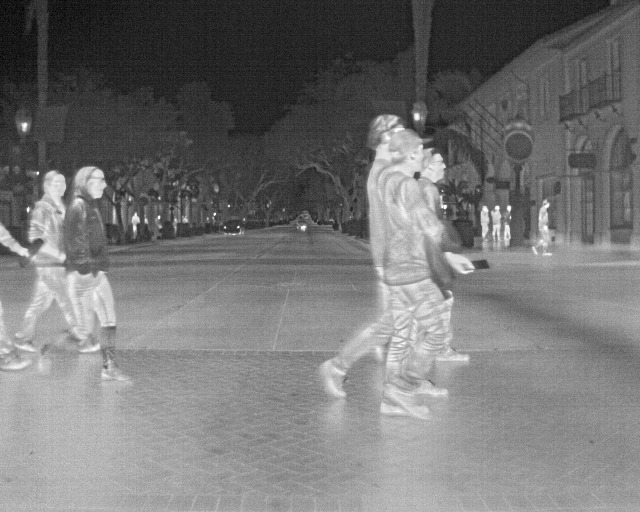
\includegraphics[width=\textwidth]{foto1presentar.jpg}
				\captionof{figure}{Imagen térmica de ejemplo.}
			\end{column}
		\end{columns}
		
		\begin{alertblock}{Metodología YOLO}
			Divide la imagen en una rejilla $S \times S$. Es un problema de regresión para encontrar la posición del objeto y de clasificación del mismo.
		\end{alertblock}
	\end{frame}
	
	% --- Sección 2: Fundamentos ---
	\section{Fundamentos de YOLO}
	\subsection{Descripción de la Neurona}
	\begin{frame}{Índice}
		\tableofcontents[currentsubsection] 
	\end{frame}
	
	\begin{frame}{La Neurona Convolucional en YOLO}
		Unidad básica de procesamiento. Hiperparámetros clave: $k$ (kernel), $P$ (padding), $S$ (stride).
		\vspace{0.2cm}
		\begin{figure}
			\centering
			\resizebox{0.9\linewidth}{!}{
				\begin{tikzpicture}[
					font=\sffamily,
					>=Latex,
					% Define styles for the blocks
					block/.style={
						draw=blue!60!black, 
						fill=blue!5, 
						thick, 
						minimum height=1.5cm, 
						minimum width=2cm, 
						align=center,
						rounded corners=3pt,
						drop shadow
					},
					sum/.style={
						circle, 
						draw=black, 
						fill=white, 
						thick, 
						inner sep=0pt, 
						minimum size=0.8cm,
						drop shadow
					},
					label_text/.style={
						font=\footnotesize\color{gray!40!black}, 
						align=center
					},
					dim_text/.style={
						font=\small\bfseries\color{blue!40!black}
					}
					]
					
					% --- 1. INPUT ---
					\node (input) at (0,0) {\Large $X$};
					\node[label_text, above=0.2cm of input] {Input Image};
					\node[below=0.5cm of input] (dim_text) {$1 \times 3 \times 640 \times 640$};
					
					% Annotation for Batch/Channels
					\draw[->, gray, thin] (dim_text.south west) ++(0.2,-1.2) -- ++(0,1.3);
					\draw[->, gray, thin] (dim_text.south west) ++(0.8,-0.8) -- ++(0,0.9);
					\draw[->, gray, thin] (dim_text.south west) ++(1.6,-0.5) -- ++(0,0.6);			
					\draw[->, gray, thin] (dim_text.south west) ++(2.6,-0.8) -- ++(0,0.9);		
					
					\node[font=\small, anchor=north] at ([xshift=0.2cm,  yshift=-1.2cm]dim_text.south west) {Batch (Imágenes)};
					\node[font=\small, anchor=north] at ([xshift=0.8cm, yshift=-0.8cm]dim_text.south west) {Canales};
					\node[font=\small, anchor=north] at ([xshift=1.6cm,  yshift=-0.5cm]dim_text.south west) {Alto};
					\node[font=\small, anchor=north] at ([xshift=2.6cm,  yshift=-0.8cm]dim_text.south west) {Ancho};	
					
					% --- 2. CONVOLUTION BLOCK (W) ---
					\node[block, right=2.5cm of input] (conv) {\Large $W$};
					\draw[->, thick] (input) -- (conv);
					\node[above=0.8cm of conv, align=center] (w_dims) {
						$32 \times 3 \times 6 \times 6$
					};
					\draw[->, gray, thin] (w_dims.north west) ++(0.35, 1.2) -- ++(0,-1.2);
					\node[font=\small, anchor=south] at ([xshift=0.35cm, yshift=1.2cm]w_dims.north west) {Filtros};
					\draw[->, gray, thin] (w_dims.north west) ++(1.05, 0.6) -- ++(0,-0.6);
					\node[font=\small, anchor=south] at ([xshift=1.05cm, yshift=0.6cm]w_dims.north west) {Canales};
					\draw[decorate, decoration={brace, amplitude=3pt, mirror}, red!60!black, thick] 
					([xshift=1.35cm, yshift=0.1cm]w_dims.south west) -- 
					([xshift=2.35cm, yshift=0.1cm]w_dims.south west);
					\node[font=\small, red!60!black, anchor=north] at ([xshift=1.95cm, yshift=0.0cm]w_dims.south west) {Kernel};
					\draw[->, thick] (w_dims) -- (conv);
					\node[label_text, below=0.2cm of conv] {Convolución con los pesos $W$};
					
					
					% --- 3. SUMMATION (Bias) ---
					\node[sum, right=1.5cm of conv] (adder) {\Large $+$};
					
					% Arrow Conv -> Sum
					\draw[->, thick] (conv) -- node[above, font=\small] {$X*W$} (adder);
					
					% Bias Input
					\node[below=1.5cm of adder] (bias) {$b = (32 \times 1)$};
					\draw[decorate, decoration={brace, amplitude=4pt, mirror}, thick, black] 
					(bias.south west) -- (bias.south east) 
					node[midway, below=4pt, font=\small\normalfont, text=black] {Sesgo};
					\draw[->, thick] (bias) -- (adder);
					
					
					% --- 4. ACTIVATION (SiLU) ---
					\node[block, right=1.5cm of adder, minimum width=1.5cm] (silu) {SiLU\\ $\sigma(\cdot)$};
					\node[label_text, below=0.2cm of silu] {Función de activación};
					% Arrow Sum -> SiLU
					\draw[->, thick] (adder) -- (silu);
					
					
					% --- 5. OUTPUT ---
					\node[right=2.5cm of silu] (output) {\Large $f(X)$};
					
					% Arrow SiLU -> Output
					\draw[->, thick] (silu) -- (output);
					
					% Output Dimensions
					\node[dim_text, below=0.6cm of output, font=\small, text=black](dim_text_2) {$1 \times 32 \times 320 \times 320$};
					\node[label_text, above=0.2cm of output] {Espacio de características};
					
					% Annotation for Batch/Channels
					\draw[->, gray, thin] (dim_text_2.south west) ++(0.8,-1.2) -- ++(0,1.3);
					\draw[->, gray, thin] (dim_text_2.south west) ++(0.2,-0.8) -- ++(0,0.9);
					\draw[->, gray, thin] (dim_text_2.south west) ++(1.6,-0.5) -- ++(0,0.6);			
					\draw[->, gray, thin] (dim_text_2.south west) ++(2.6,-0.8) -- ++(0,0.9);		
					
					\node[font=\small, anchor=north] at ([xshift=0.2cm,  yshift=-0.8cm]dim_text_2.south west) {Batch };
					\node[font=\small, anchor=north] at ([xshift=0.8cm, yshift=-1.2cm]dim_text_2.south west) {Características};
					\node[font=\small, anchor=north] at ([xshift=1.6cm,  yshift=-0.5cm]dim_text_2.south west) {Alto};
					\node[font=\small, anchor=north] at ([xshift=2.6cm,  yshift=-0.8cm]dim_text_2.south west) {Ancho};	
					
				\end{tikzpicture}
			}
			\caption{Estructura de la neurona a la entrada.}
		\end{figure}
	\end{frame}
	
	\begin{frame}{Ecuaciones del modelo: Convolución y Dimensiones}
		\textbf{Operación de Convolución 2D:}
		\begin{itemize}
			\item Implementada técnicamente como correlación cruzada (sin voltear el kernel):
		\end{itemize}
		
		\begin{equation}
			(W * X)(c_{out}, h, w) = \sum_{l=0}^{C_{in}-1} \sum_{i=0}^{K_H-1} \sum_{j=0}^{K_W-1} W(c_{out}, l, i, j) \cdot X(l, h \cdot S + i \cdot d , w \cdot S + j \cdot d)
		\end{equation}
		
		\vfill
		
		\textbf{Dimensiones del mapa de características de salida:}
		\begin{itemize}
			\item Relación generalizada considerando el factor de dilatación $d$:
		\end{itemize}
		
		\begin{equation}
			Out = \left\lfloor \frac{In + 2P}{S} \right\rfloor + 1
		\end{equation}
	\end{frame}
	
	\begin{frame}{Función de Activación: SiLU}
		\begin{columns}
			\column{0.5\textwidth}
			\textbf{Sigmoid Linear Unit (SiLU):}
			\begin{equation}
				f(z) = z \cdot \sigma(z) = \frac{z}{1+e^{-z}}
			\end{equation}
			\begin{itemize}
				\item Permite flujo de gradientes en valores negativos pequeños.
				\item Suavidad superior a ReLU.
				\item Mejora la convergencia en redes profundas.
			\end{itemize}
			
			\column{0.5\textwidth}
			\begin{figure}
				\centering
				\resizebox{0.95\linewidth}{!}{
					\begin{tikzpicture}
						\begin{axis}[
							axis lines=middle, xlabel={$z$}, ylabel={$f(z)$},
							grid=major, width=10cm, height=8cm,
							xmin=-4.5, xmax=4.5, ymin=-1, ymax=4.5,
							title={Gráfica de SiLU}
							]
							\addplot[color=blue!70!black, ultra thick, domain=-4.5:4.5, samples=100] {x / (1 + exp(-x))};
						\end{axis}
					\end{tikzpicture}
				}
			\end{figure}
		\end{columns}
	\end{frame}
	
	% --- Sección 3: Topología ---
	\subsection{Topología de la Red}
	\begin{frame}{Índice}
		\tableofcontents[currentsubsection] 
	\end{frame}
	\begin{frame}{Bloque ResNet (Residual Network)}
		\begin{itemize}
			\item \textbf{Problema:} Gradientes explotan/desvanecen en redes muy profundas.
			\item \textbf{Solución:} Conexión identidad. $y = \mathcal{F}(x) + x$.
		\end{itemize}
		\vspace{0.2cm}
		\begin{figure}
			\centering
			\resizebox{0.6\linewidth}{!}{
				\begin{tikzpicture}[
					node distance=1.5cm,
					% --- Styles ---
					cvblock/.style={
						rectangle, draw, rounded corners, fill=cyan!10, drop shadow,
						minimum width=1.2cm, minimum height=1.2cm, align=center, font=\bfseries\sffamily\scriptsize
					},
					% Rhombus Style for Sumator
					sumnode/.style={
						diamond, draw, fill=green!10, drop shadow,
						minimum width=1.0cm, minimum height=1.0cm, align=center, font=\bfseries\sffamily\large, inner sep=0pt
					},
					line/.style={
						draw, -Latex, thick, color=darkgray
					},
					dimlabel/.style={
						font=\sffamily\tiny, color=gray, align=center, auto
					}
					]
					
					% --- 1. Input Node (Invisible start point) ---
					\node (input_start) {};
					
					% --- 2. Main Processing Branch (Top) ---
					% First CV
					\node [cvblock, right=2cm of input_start] (cv1) {CV\\$W_{A}$};
					
					% Second CV
					\node [cvblock, right=1.2cm of cv1] (cv2) {CV\\$W_{B}$};
					
					% Sumator (Rhombus)
					\node [sumnode, right=1.2cm of cv2, label=below:\sffamily\scriptsize] (sigma) {$\Sigma$};
					
					% --- 3. Connections & Shortcut ---
					
					% Input Line
					\draw [line] (input_start) -- (cv1.west);
					
					% Label Input Size
					\node [dimlabel, above] at ($(input_start)!0.5!(cv1.west)$) {Tamaño Entrada\\$C \times H \times W$};
					
					% Internal Connections (Main Branch)
					\draw [line] (cv1) -- node[dimlabel, above] {} (cv2);
					\draw [line] (cv2) -- (sigma.west);
					
					% --- The Residual Shortcut (The "Loop") ---
					% Define a split point before CV1
					\coordinate (split_point) at ($(cv1.west) + (-1.0, 0)$);
					
					% Define the target at the BOTTOM of the diamond
					\coordinate (sigma_bottom) at (sigma.south);
					
					% Draw Shortcut Line:
					% 1. Start at split point
					% 2. Go Down (vertical)
					% 3. Go Right (horizontal) until under the sigma
					% 4. Go Up into the sigma
					% --- The Residual Shortcut (The "Loop") ---
					\coordinate (split_point) at ($(cv1.west) + (-1.0, 0)$);
					\coordinate (sigma_bottom) at (sigma.south);
					
					% 1. The Line (Clean)
					\draw [line] (split_point) -- ++(0, -1.8) -| (sigma_bottom);
					
					% 2. The Text (Separated)
					% Logic: Located halfway (0.5) horizontally between start and end, 
					% and shifted down 1.8cm to match the line's depth.
					\node [font=\sffamily\tiny, color=gray, below, yshift=-2pt] 
					at ($(split_point)!0.5!(sigma) + (0, -1.8)$) 
					{Identidad (Residuos)};
					
					
					% Dot
					\fill [darkgray] (split_point) circle (2pt);
					% Add the visual "dot" at the split point for clarity
					\fill [darkgray] (split_point) circle (2pt);
					
					% --- 4. Final Output ---
					\node [right=1.5cm of sigma] (output_end) {};
					\draw [line] (sigma.east) -- (output_end);
					
					% Label Output Preservation
					\node [dimlabel, above] at ($(sigma.east)!0.5!(output_end)$) {Tamaño Salida\\$C \times H \times W$\\(Preservada)};
					
					% --- 5. Legend ---
					\node [draw, dashed, fill=white, rounded corners, 
					font=\sffamily\scriptsize, align=left, anchor=north,
					% CHANGE THE NUMBERS BELOW TO MOVE THE BOX: (X, Y)
					at={($(cv2) + (-0.5, -2.2)$)}] {
						\textbf{Leyenda:}\\
						\textbf{CV}: Capa convolucional.\\
						\textbf{$\Sigma$}: Suma elemento a elemento.\\
						\textbf{C}: Número de canales.\\
						\textbf{H,W}: Ancho y alto de los mapas de características.\\
						$W_{A}=\{C, C, 1, 1\}$: Pesos capa de entrada que reduce/procesa canales.\\
						$W_{B}=\{C, C, 3, 3\}$: Pesos capa de extracción características.
					};
					
				\end{tikzpicture}
			}
			\caption{Arquitectura Bloque ResNet: Aprende $F(x)$ (ruido/características) sobre la identidad.}
		\end{figure}
	\end{frame}
	
	\begin{frame}{Bloque CSP / C3 (Cross Stage Partial)}
		\begin{itemize}
			\item \textbf{Problema:} Ineficiencia por duplicidad de información en el gradiente y cálculos redundantes en redes profundas.
			\item \textbf{Solución:} Bifurcar el flujo de entrada. Una rama extrae características complejas mientras la otra preserva el contexto global. $y = \mathcal{T}[\mathcal{F}(x) \parallel \mathcal{G}(x)]$
		\end{itemize}
		
		
		\begin{figure}
			\centering
			\resizebox{0.6\linewidth}{!}{
				\begin{tikzpicture}[
					node distance=1.5cm,
					% --- Styles ---
					cvblock/.style={
						rectangle, draw, rounded corners, fill=cyan!10, drop shadow,
						minimum width=1.2cm, minimum height=1.2cm, align=center, font=\bfseries\sffamily\scriptsize
					},
					concatblock/.style={
						rectangle, draw, fill=orange!20, drop shadow,
						minimum width=1cm, minimum height=3.5cm, align=center, font=\bfseries\sffamily\small
					},
					line/.style={
						draw, -Latex, thick, color=darkgray
					},
					dimlabel/.style={
						font=\sffamily\tiny, color=gray, align=center, auto
					}
					]
					
					% --- 1. Entry Concatenator ---
					\node [concatblock, label=below:\sffamily\scriptsize In Concat] (concat_in) {CONCAT};
					
					% Inputs to Entry Concat
					\draw [line] ($(concat_in.west) + (-2, 0.5)$) -- node[above, font=\tiny] {In 1} ($(concat_in.west) + (0, 0.5)$);
					\draw [line] ($(concat_in.west) + (-2, -0.5)$) -- node[below, font=\tiny] {In 2} ($(concat_in.west) + (0, -0.5)$);
					
					% --- 2. Top Branch (Main Processing: 3 CVs) ---
					% Position relative to entry concat
					\node [cvblock, above right=0.0cm and 1.5cm of concat_in] (top1) {CV\\$W_{1}$};
					\node [cvblock, right=0.8cm of top1] (top2) {CV\\$W_{2}$};
					\node [cvblock, right=0.8cm of top2] (top3) {CV\\$W_{3}$};
					
					% --- 3. Bottom Branch (Shortcut: 1 CV) ---
					% Positioned centrally below the top chain for symmetry
					% We align it horizontally with top2 so it looks balanced
					\node [cvblock, below=3.5cm of top2] (bot1) {CV\\$W_{1}$};
					
					% --- Connections from Entry Concat to Branches ---
					\coordinate (split_point) at ($(concat_in.east) + (0.5, 0)$);
					
					% 1. Draw the line (Clean, no text)
					\draw [line] (concat_in.east) -- (split_point);
					
					% 2. Draw the text (Separately)
					% We place it exactly halfway (0.5) between concat_in and split_point
					\node [dimlabel, above, yshift=-6pt] at ($(concat_in.east)!2.6!(split_point)$) {$2C \times H \times W$};
					
					\node [dimlabel, above, yshift=-8pt] at ($(concat_in.east)!-6!(split_point)$) {Tamaño Entrada\\$C \times H \times W$};
					
					% To Top (No text)
					\draw [line] (split_point) |- (top1.west);
					
					% To Bottom (No text)
					\draw [line] (split_point) |- (bot1.west);
					
					% --- Connections within branches ---
					% Top chain
					\draw [line] (top1) -- (top2);
					\draw [line] (top2) -- (top3);
					
					% --- 4. Output Concatenator ---
					\node [concatblock, right=9cm of concat_in, label=below:\sffamily\scriptsize Out Concat] (concat_out) {CONCAT};
					
					
					
					% FIX: Define a shared vertical axis for the bend (0.8cm to the right of top3)
					% This ensures both lines turn at the exact same X-coordinate
					\coordinate (turn_axis) at ($(top3.east) + (0.8, 0)$);
					
					% Connect Top Branch (Path 1)
					\coordinate (in_top) at ($(concat_out.west) + (0, 0.6)$);
					
					% Draw: (Start) -- (Go to Axis) |- (Target)
					% The syntax (source -| turn_axis) finds the intersection point (axis X, source Y)
					\draw [line] (top3.east) -- (top3.east -| turn_axis) |- (in_top) node[left, font=\tiny, xshift=-2pt,yshift=-5pt] {(1)}; 
					
					% Connect Bottom Branch (Path 2)
					\coordinate (in_bot) at ($(concat_out.west) + (0, -0.6)$);
					
					% Draw: Same logic, it will extend the line further to hit the same axis
					\draw [line] (bot1.east) -- (bot1.east -| turn_axis) |- (in_bot) node[left, font=\tiny, xshift=-2pt,yshift=5pt] {(2)};
					% --- Legend / Info Box ---
					% --- 5. Final Transition & Output ---
					% Add the final CV block after Concat
					\node [cvblock, right=1.0cm of concat_out] (final_cv) {CV\\$W_{4}$};
					\draw [line] (concat_out.east) -- (final_cv.west);
					
					% Draw the final outgoing line
					\node [right=1.5cm of final_cv] (final_out) {};
					\draw [line] (final_cv.east) -- (final_out);
					
					% Label the preservation of size at the very end
					\node [dimlabel, above] at ($(final_cv.east)!0.5!(final_out)$) {Tamaño Salida\\$C \times H \times W$\\(Preservada)};
					
					\node [draw, dashed, fill=white, rounded corners, below=0.5cm of bot1, font=\sffamily\scriptsize, align=left] {
						\textbf{Leyenda:}\\
						\textbf{CV}: Capa convolucional.\\
						\textbf{Concat}: Concatenador de cadenas.\\
						\textbf{C}: Número de canales.\\
						\textbf{H,W}: Ancho y alto de los mapas de características.\\
						$W_{1}=\{C/2,2C,1,1\}$: Pesos capa de entrada que comprimen la información de los canales de entrada.\\
						$W_{2}=\{C/2,C/2,1,1\}$: Pesos capa de compresión de dimensiones antes de la extracción de características.\\
						$W_{3}=\{C/2,C/2,3,3\}$: Pesos capa de extracción de características.\\
						$W_{4}=\{C,C,1,1\}$: Pesos capa de salida para combinar la información de las características extraídas.
					};
					
				\end{tikzpicture}
			}
			\caption{Bloque CSP: Mejora la variabilidad del aprendizaje reduciendo la redundancia.}
		\end{figure}
	\end{frame}
	
\begin{frame}{Bloque C3-k (CSPResNe(X)t)}
	\begin{itemize}
		\item \textbf{Problema:} Necesidad de aumentar la profundidad de la red para extraer características complejas sin sufrir degradación del gradiente.
		\item \textbf{Solución:} Sustituir convoluciones simples por una serie de $k$ bloques \textbf{ResNet} en la rama profunda de la arquitectura CSP.
	\end{itemize}
	
	\begin{figure}
		\centering
		\resizebox{0.7\linewidth}{!}{
				\begin{tikzpicture}[
				node distance=1.5cm,
				% --- Styles ---
				cvblock/.style={
					rectangle, draw, rounded corners, fill=cyan!10, drop shadow,
					minimum width=1.2cm, minimum height=1.2cm, align=center, font=\bfseries\sffamily\scriptsize
				},
				resnetblock/.style={
					rectangle, draw, fill=yellow!20, rounded corners, drop shadow,
					minimum width=1.5cm, minimum height=1.2cm, align=center, font=\bfseries\sffamily\scriptsize
				},
				concatblock/.style={
					rectangle, draw, fill=orange!20, drop shadow,
					minimum width=1cm, minimum height=3.5cm, align=center, font=\bfseries\sffamily\small
				},
				line/.style={
					draw, -Latex, thick, color=darkgray
				},
				dimlabel/.style={
					font=\sffamily\tiny, color=gray, align=center, auto
				}
				]
				
				% --- 1. Entrada y CV Inicial ---
				\node (input_start) {};
				
				% CV de Entrada (NUEVO)
				\node [cvblock] (cv_in) at (0,0) {CV\\$W_{1}$};
				
				% Línea desde "nada" hasta CV in
				\draw [line] ($(cv_in.west) + (-1.5, 0)$) -- node[dimlabel, above] {} (cv_in.west);
				\node [font=\sffamily\tiny, color=gray, below] 
				at ($(split_point)!0.5!(sigma_bottom) + (-5.8, 0.75)$) 
				{$C\times H \times W$};
				
				\node [font=\sffamily\tiny, color=gray, below] 
				at ($(split_point)!0.5!(sigma_bottom) + (-2.8, 0.75)$) 
				{$2C\times H/2 \times W/2$};
				% --- 2. Punto de División (Split) ---
				% El punto de split está justo a la salida de la CV de entrada
				\coordinate (split_point) at ($(cv_in.east) + (2.0, 0)$);
				\draw [line] (cv_in.east) -- (split_point);
				
				
				% --- 3. Rama Superior (Procesamiento) ---
				% CV Rama Superior
				\node [cvblock, above right=0.5cm and 1.0cm of split_point] (top_cv) {CV\\$W_{2}$};
				
				% ResNet Bloque 1
				\node [resnetblock, right=0.8cm of top_cv] (res1) {Bloque\\ResNet};
				
				% ResNet Bloque 2
				\node [resnetblock, right=1.0cm of res1] (res2) {Bloque\\ResNet};
				
				% Conexiones Superiores
				\draw [line] (split_point) |- (top_cv.west);
				\draw [line] (top_cv) -- (res1);
				
				% FLECHA PUNTEADA ENTRE RESNETS (NUEVO)
				\draw [line, dashed] (res1) -- (res2);
				
				% Llave indicando k veces
				\draw [decorate, decoration={brace, amplitude=6pt, raise=4pt}, thick, color=darkgray]
				(res1.north west) -- (res2.north east)
				node [midway, above=10pt, font=\sffamily\scriptsize\bfseries] {$\times k$ veces};
				
				
				% --- 4. Rama Inferior (Atajo) ---
				% CV Rama Inferior
				\node [cvblock, below right=0.5cm and 1.0cm of split_point] (bot_cv) {CV\\$W_{2}$};
				
				% Conexión Inferior
				\draw [line] (split_point) |- (bot_cv.west);
				
				
				% --- 5. Concatenación de Salida ---
				\node [concatblock, right=1.5cm of res2, yshift=-1.1cm, label=below:\sffamily\scriptsize ] (concat_out) {CONCAT};
				
				% Ejes de giro para flechas simétricas
				\coordinate (turn_axis) at ($(res2.east) + (0.8, 0)$);
				
				% Conexión Superior (1)
				\coordinate (in_top) at ($(concat_out.west) + (0, 0.6)$);
				\draw [line] (res2.east) -- (res2.east -| turn_axis) |- (in_top) node[left, font=\tiny, xshift=-2pt,yshift=-5pt] {(1)}; 
				
				% Conexión Inferior (2)
				\coordinate (in_bot) at ($(concat_out.west) + (0, -0.6)$);
				\draw [line] (bot_cv.east) -- (bot_cv.east -| turn_axis) |- (in_bot) node[left, font=\tiny, xshift=-2pt,yshift=5pt] {(2)};
				
				
				% --- 6. CV Final y Salida ---
				\node [cvblock, right=1.0cm of concat_out] (final_cv) {CV\\$W_{3}$};
				\draw [line] (concat_out.east) -- (final_cv.west);
				
				\node [right=1.5cm of final_cv] (final_out) {};
				\draw [line] (final_cv.east) -- (final_out);
				\node [dimlabel, above] at ($(final_cv.east)!0.7!(final_out)$) {Salida\\$2C\times H/2 \times W/2$};
				
				
				% --- 7. Leyenda ---
				\node [draw, dashed, fill=white, rounded corners, font=\sffamily\scriptsize, align=left, anchor=north, at={($(bot_cv) + (2.5, -1.3)$)}] {
					\textbf{Leyenda:}\\
					\textbf{CV}:  Capa convolucional.\\
					\textbf{Bloque ResNet}: Módulo residual repetido \(k\) veces\\
					\textbf{C}: Número de canales.\\
					\textbf{H,W}: Ancho y alto de los mapas de características.\\
					$W_{1}=\{2C,C,3,3\}$: Pesos capa de entrada para una extracción preliminar de características\\
					$W_{2}=\{C,2C,1,1\}$: Pesos capa intermedia para la compresión de canales.\\
					$W_{3}=\{2C,2C,1,1\}$: Pesos capa de salida para combinar la información de la rama de extracción de características con el mapa de características orignal.
				};
				
			\end{tikzpicture}
		}
	\caption{Bloque C3-k: Mejora del aprendizaje para no sufrir degradación del gradiente.}
	\end{figure}
\end{frame}
	
	\begin{frame}{Bloque SPPF (Spatial Pyramid Pooling Fast)}
\begin{itemize}
	\item \textbf{Problema:} Capturar contexto multiescala sin el coste computacional de kernels grandes en paralelo.
	\item \textbf{Solución:} Estructura en \textbf{cascada} de Max Pooling ($5\times5$). Tres capas en serie equivalen matemáticamente a un kernel grande.
	\item \textbf{Invarianza:} El Max Pooling extrae la característica dominante, otorgando robustez ante  traslaciones y deformaciones del objeto.
\end{itemize}
		
		\begin{columns}
			% --- COLUMNA IZQUIERDA: Diagrama TikZ ---
			\column{0.3\textwidth}
			\begin{figure}
				\centering
				\resizebox{1\linewidth}{!}{
					\begin{tikzpicture}[
						node distance=1.0cm,
						cvblock/.style={rectangle, draw, rounded corners, fill=cyan!10, drop shadow, minimum width=1.5cm, minimum height=1.2cm, align=center, font=\bfseries\sffamily\scriptsize},
						mpblock/.style={rectangle, draw, rounded corners, fill=red!15, drop shadow, minimum width=1.5cm, minimum height=1.2cm, align=center, font=\bfseries\sffamily\scriptsize},
						concatblock/.style={rectangle, draw, fill=orange!20, drop shadow, minimum width=1.2cm, minimum height=7.5cm, align=center, font=\bfseries\sffamily\small},
						line/.style={draw, -Latex, thick, color=darkgray},
						dimlabel/.style={font=\sffamily\tiny, color=gray, align=center, auto},
						dot/.style={circle, fill=darkgray, inner sep=0pt, minimum size=4pt}
						]
						
						\node [cvblock] (cv_in) {CV\\$W_{1}$};
						\node [mpblock, below=1.0cm of cv_in, xshift=2.0cm] (mp1) {MP\\$k=5$};
						\node [mpblock, below=1.0cm of mp1, xshift=2.0cm] (mp2) {MP\\$k=5$};
						\node [mpblock, below=1.0cm of mp2, xshift=2.0cm] (mp3) {MP\\$k=5$};
						
						\node [concatblock, right=4.5cm of $(cv_in)!0.5!(mp3)$] (concat_out) {{CONCAT}};
						
						\coordinate (port1) at (cv_in -| concat_out.west);
						\coordinate (port2) at (mp1 -| concat_out.west);
						\coordinate (port3) at (mp2 -| concat_out.west);
						\coordinate (port4) at (mp3 -| concat_out.west);
						
						\draw [line] (cv_in.east) -- (port1);
						\coordinate (split1) at ($(mp1.north) + (0, 1.6)$); 
						\node [dot] at (split1) {};
						\draw [line] (split1) -- (mp1.north);
						
						\draw [line] (mp1.east) -- (port2);
						\coordinate (split2) at ($(mp2.north) + (0, 1.6)$);
						\node [dot] at (split2) {};
						\draw [line] (split2) -- (mp2.north);
						
						\draw [line] (mp2.east) -- (port3);
						\coordinate (split3) at ($(mp3.north) + (0, 1.6)$);
						\node [dot] at (split3) {};
						\draw [line] (split3) -- (mp3.north);
						
						\draw [line] (mp3.east) -- (port4);
						
						\node [cvblock, right=1.0cm of concat_out] (cv_out) {CV\\$W_{2}$};
						\draw [line] (concat_out.east) -- (cv_out.west);
					\end{tikzpicture}
				}
				\caption{Arquitectura SPPF.}
			\end{figure}
			
			% --- COLUMNA DERECHA: Imagen Externa ---
			\column{0.3\textwidth}
			\begin{figure}
				\centering
				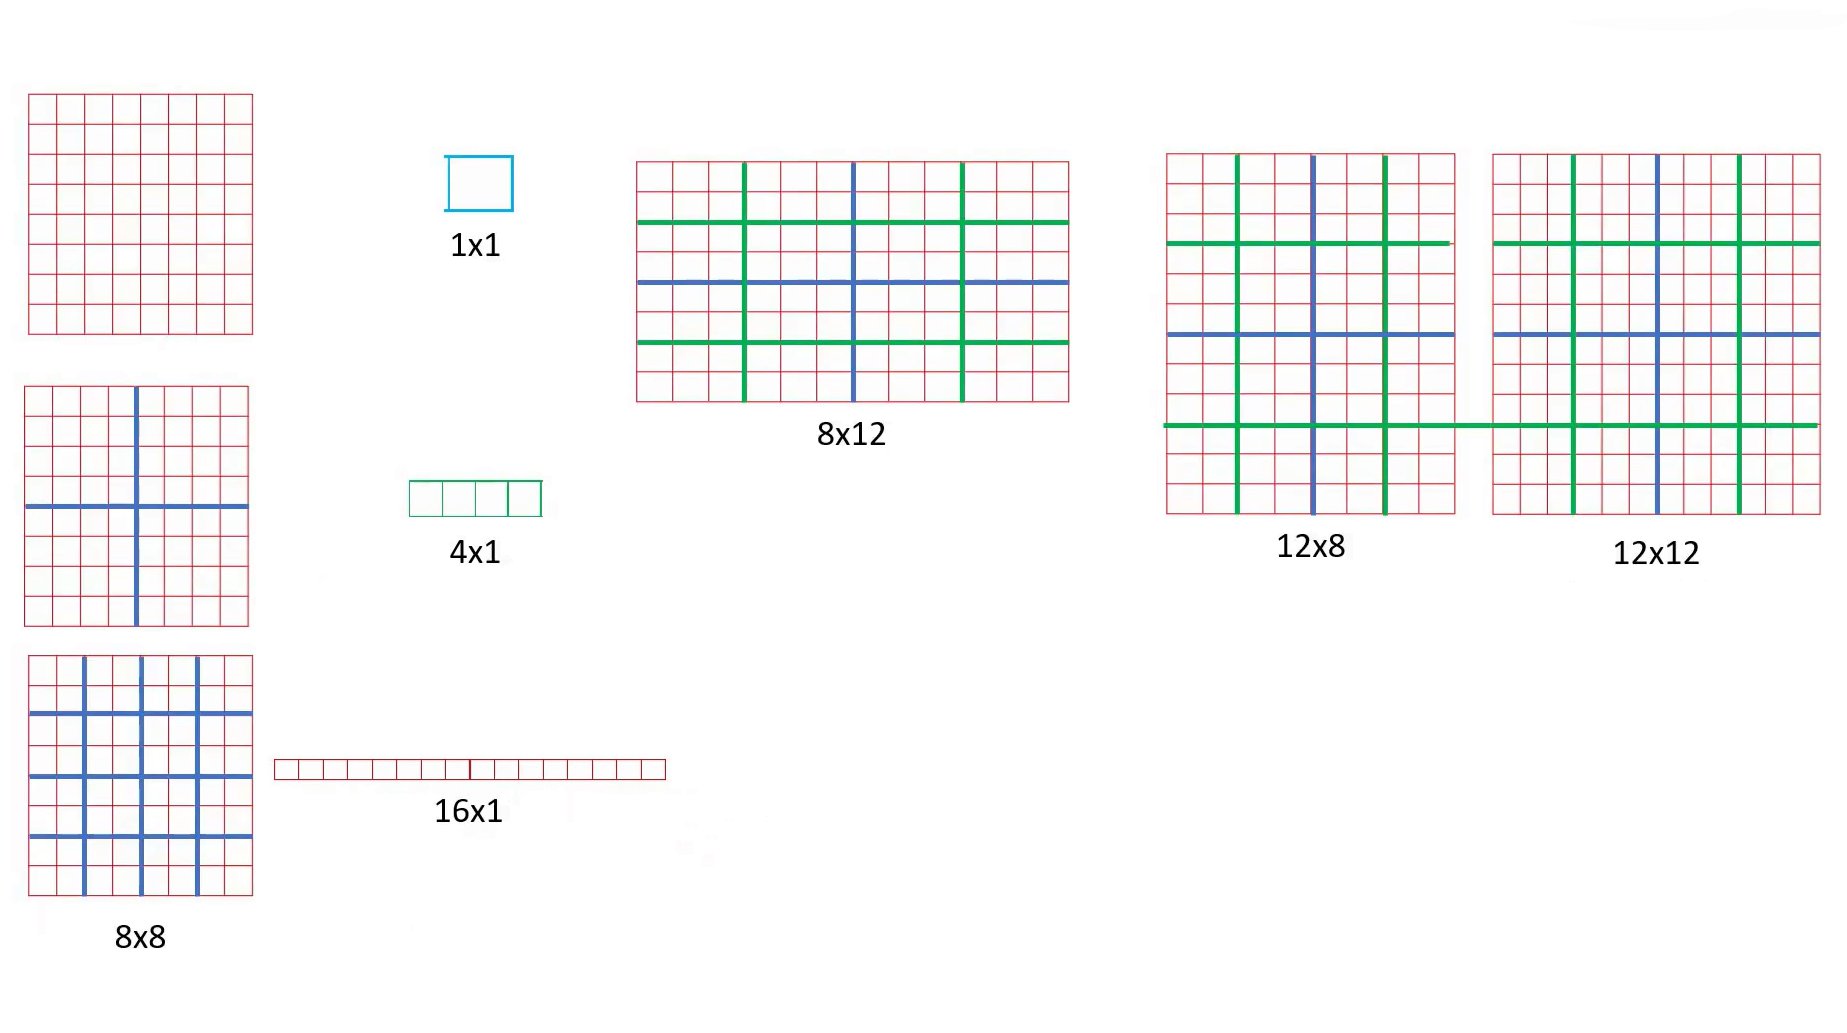
\includegraphics[width=1\linewidth]{indioVidio}
				\caption{Ejemplo del comportamiento invariante.}
			\end{figure}
		\end{columns}
	\end{frame}

\begin{frame}{Cabeza de Detección (Head)}
	% --- Texto en la parte superior ---
	\begin{itemize}
		\item \textbf{Multiescala:} 3 ramas de detección ($i=\{1,2,3\}$) para diferentes tamaños de objeto.
		\item \textbf{Salidas por anclaje:}
		\begin{enumerate}
			\item Coordenadas de la caja delimitadora ($t_x, t_y, t_w, t_h$).
			\item Probabilidad de objeto.
			\item Probabilidades de clasificación por categoría.
		\end{enumerate}
		\item \textbf{Arquitectura:} Red totalmente convolucional (FCN) sin capas densas.
	\end{itemize}
	
	\vfill % Espacio elástico para separar texto de imagen
	
	% --- Figura en la parte inferior ---
	\begin{figure}
		\centering
		\resizebox{0.95\linewidth}{!}{
						\begin{tikzpicture}[
				node distance=1.5cm and 2.0cm, 
				% --- ESTILOS ---
				cvblock/.style={
					rectangle, draw, rounded corners, fill=cyan!10, drop shadow,
					minimum width=2.0cm, minimum height=1.2cm, align=center, font=\bfseries\sffamily\scriptsize
				},
				concatblock/.style={
					rectangle, draw, fill=orange!20, drop shadow,
					minimum width=1.2cm, minimum height=4.5cm, align=center, font=\bfseries\sffamily\small
				},
				opnode/.style={
					circle, draw, fill=gray!10, drop shadow, thick,
					minimum size=1.2cm, align=center, font=\bfseries\sffamily\large
				},
				line/.style={
					draw, -Latex, thick, color=darkgray, rounded corners=5pt
				},
				dimlabel/.style={
					font=\sffamily\tiny, color=darkgray, align=center, auto, fill=white, inner sep=1pt
				},
				dot/.style={
					circle, fill=darkgray, inner sep=0pt, minimum size=4pt
				}
				]
				
				% ==========================================
				% 1. Entrada y Convolución Inicial (Wi)
				% ==========================================
				\node (input_i) at (0,0) {\Large $i$};
				\node [opnode, right=1.0cm of input_i] (wi_node) {$W_i$};
				\draw [line] (input_i) -- (wi_node);
				
				% ==========================================
				% 2. Primer Reshape y Activación
				% ==========================================
				\node [cvblock, right=3.0cm of wi_node] (reshape1) {Reshape};
				\draw [line] (wi_node) -- node[dimlabel] {$1 \times 255 \times H \times W$} (reshape1);
				
				\node [opnode, right=1.5cm of reshape1] (sigma_node) {$\sigma$};
				\draw [line] (reshape1) -- coordinate (mid) (sigma_node);
				\draw [thin, darkgray] (mid) -- ++(0, 0.6) node[dimlabel, anchor=south] {$3 \times H \times W \times 85$};
				
				% ==========================================
				% 3. División en 3 Ramas y Primer Concat
				% ==========================================
				\node [concatblock, right=6.0cm of sigma_node] (concat1) {Concat};
				
				% --- MODIFICATION START ---
				
				% 1. Define Coords block to span Middle (y=0) and Bottom (y=-1.5)
				% We position it halfway horizontally, and shift it down by 0.75cm vertically
				% We also increase height to 2.5cm to cover both "lanes"
				\node [cvblock, minimum height=2.8cm] (coords) at ($(sigma_node)!0.5!(concat1) + (0, -0.75)$) {Coords};
				
				% 2. Split Point
				\coordinate (split_sigma) at ($(sigma_node.east) + (1.0, 0)$);
				\draw [line] (sigma_node) -- (split_sigma);
				\node [dot] at (split_sigma) {};
				
				% 3. Concat Inputs
				\coordinate (concat1_in1) at ($(concat1.west) + (0, 1.5)$);
				\coordinate (concat1_in2) at (concat1.west); % Middle input
				\coordinate (concat1_in3) at ($(concat1.west) + (0, -1.5)$); % Bottom input
				
				% --- Branch 1: Top (Classes) ---
				\draw [line] (split_sigma) |- (concat1_in1) 
				node[dimlabel, pos=0.7] {$3 \times H \times W \times 81$} 
				node[at end, left, font=\tiny, xshift=-3pt,yshift=5] {1};
				
				% --- Branches 2 & 3: Coords & Objectness (Going through the big block) ---
				
				% Labels centered on the block (between the lines)
				%\node [dimlabel] at ($(split_sigma)!0.5!(coords.west)$) {$3 \times H \times W \times 4$};
				\node [dimlabel] at ($(coords.east)!0.5!(concat1.west |- coords.east)$) {$3 \times H \times W \times 4$};
				
				% Drawing the lines passing through
				% Middle Line (Branch 2)
				\draw [line] (split_sigma) -- (split_sigma |- coords.west) -- (coords.west |- split_sigma); % Enters block
				\draw [line] (coords.east |- concat1_in2) -- (concat1_in2) node[at end, left, font=\tiny, xshift=-3pt,yshift=5] {2}; % Exits block
				
				% Bottom Line (Branch 3)
				\draw [line] (split_sigma) |- (coords.west |- concat1_in3); % Enters block
				\draw [line] (coords.east |- concat1_in3) -- (concat1_in3) node[at end, left, font=\tiny, xshift=-3pt,yshift=5] {3}; % Exits block
				
				% --- MODIFICATION END ---
				
				% ==========================================
				% 4. Segundo Reshape y Concat Final
				% ==========================================
				\node [cvblock, right=1.5cm of concat1] (reshape2) {Reshape};
				\draw [line] (concat1) -- (reshape2);
				
				\node [concatblock, right=2.0cm of reshape2, minimum height=2.5cm] (concat2) {\(\text{Concat}_{\text{i}}\)};
				\draw [line] (reshape2) -- (concat2.west);
				
				% Linea de retorno 'i'
				
				
				% ==========================================
				% 5. Salida Final
				% ==========================================
				\node [right=1.5cm of concat2] (final_out) {};
				\draw [line] (concat2.east) -- (final_out) node[midway, above, font=\sffamily\scriptsize,xshift=-80] {$K_i \times 85$};
				\path (concat2.east) -- (final_out) node[midway, above, font=\sffamily\scriptsize] {Salida};
				
				\node [draw, dashed, fill=white, rounded corners, font=\sffamily, align=left, anchor=north, at={($(coords) + (0, -2)$)}] {
					\textbf{Leyenda:}\\
					$\mathbf{W}_i$:  Convolución de tamaño \(255\times i\cdot 128\times1\times1\)\\
					$\mathbf{\sigma}$: Función de activación Relu.\\
					\textbf{Reshape}: Bloque que transforma las dimensiones de los tensores.\\
					\textbf{Coords}: Bloque encargado de realizar las operaciones necesarias para transformar a coordenadas absolutas.\\
					\textbf{Concat}: Concatenador de cadenas.
				};
			\end{tikzpicture}
		}
		\caption{Esquema de la Cabeza de Detección: Procesamiento de tensores para predicción multiescala.}
	\end{figure}
\end{frame}
	
	% --- Slide Especial: Arquitectura Global ---
	\begin{frame}[plain]
		\begin{center}
			\textbf{Arquitectura Global YOLO: Backbone + Neck + Head}
			\vspace{0.2cm}
			
			\resizebox{!}{0.85\textheight}{
				\begin{tikzpicture}[
					node distance=1.0cm and 1.0cm,
					% --- ESTILOS ---
					cvblock/.style={
						rectangle, draw, rounded corners, fill=cyan!10, drop shadow,
						minimum width=1.4cm, minimum height=1.0cm, align=center, font=\bfseries\sffamily\tiny
					},
					c3block/.style={ % Verde Menta (C3-K)
						rectangle, draw, rounded corners, fill=green!20, drop shadow,
						minimum width=1.4cm, minimum height=1.0cm, align=center, font=\bfseries\sffamily\tiny
					},
					sppfblock/.style={
						rectangle, draw, rounded corners, fill=red!15, drop shadow,
						minimum width=1.4cm, minimum height=1.0cm, align=center, font=\bfseries\sffamily\tiny
					},
					cspblock/.style={
						rectangle, draw, rounded corners, fill=orange!30, drop shadow,
						minimum width=1.8cm, minimum height=1.0cm, align=center, font=\bfseries\sffamily\scriptsize
					},
					resizeblock/.style={ % Fucsia Romboidal
						diamond, draw, fill=magenta!40, drop shadow, aspect=2,
						minimum width=1.6cm, minimum height=0.8cm, align=center, font=\bfseries\sffamily\tiny
					},
					headblock/.style={
						rectangle, draw, rounded corners, fill=gray!10, drop shadow,
						minimum width=12cm, minimum height=1.5cm, align=center, font=\bfseries\sffamily\normalsize
					},
					line/.style={
						draw, -Latex, thick, color=darkgray, rounded corners=4pt
					},
					dot/.style={ % Punto de soldadura
						circle, fill=darkgray, inner sep=0pt, minimum size=3.5pt
					}
					]
					
					% ==========================================
					% 1. INICIO VERTICAL (Backbone Parte 1)
					% ==========================================
					
					% Input
					\node (input) at (0,0) {};
					
					
					% Pila Vertical Izquierda
					\node [cvblock, below=0.8cm of input] (cv1) {CV\\$W_1$};
					\node [c3block, below=0.8cm of cv1] (c3_1) {C3-1};
					\node [c3block, below=0.8cm of c3_1] (c3_2) {C3-2}; % Salida P3
					
					% Conexiones Verticales
					\draw [line] (input) -- (cv1);
					\draw [line] (cv1) -- (c3_1);
					\draw [line] (c3_1) -- (c3_2);
					
					
					% ==========================================
					% 2. EXTENSIÓN HORIZONTAL (Backbone Parte 2)
					% ==========================================
					
					% Bifurcación en C3-2
					\coordinate (split_p3) at ($(c3_2.south) + (0, -0.4)$);
					\draw [thick, color=darkgray] (c3_2.south) -- (split_p3);
					\node [dot] at (split_p3) {};
					
					% Continuamos a la derecha desde la bifurcación
					% Usamos posicionamiento relativo para crear la fila superior
					% Nota: Subimos un poco para separar visualmente backbone de neck
					\node [c3block, right=1.2cm of c3_2] (c3_3) {C3-3};
					\node [c3block, right=1.0cm of c3_3] (c3_4) {C3-1}; % Salida P5 (C3-1 deep)
					\node [sppfblock, right=1.0cm of c3_4] (sppf) {SPPF};
					\node [cvblock, right=1.0cm of sppf] (cv_top) {CV\\$W_2$};
					
					% Conexión "L" (De vertical a horizontal)
					\draw [line] (split_p3) -| (c3_3.south); % Sube por abajo
					
					% Conexiones Horizontales
					\draw [line] (c3_3) -- (c3_4);
					\draw [line] (c3_4) -- (sppf);
					\draw [line] (sppf) -- (cv_top);
					
					
					% ==========================================
					% 3. NECK - BAJADA (FPN)
					% ==========================================
					
					% --- Nivel 1: Bajada P5 ---
					\node [resizeblock, below=1.2cm of cv_top] (resize1) {Resize};
					\draw [line] (cv_top.south) -- (resize1.north);
					
					% CSP Superior (Fusiona P5 + P4)
					% Lo alineamos verticalmente con C3-4 para que la bajada sea recta
					\node [cspblock, xshift=1.5cm] (csp1) at (c3_4 |- resize1) {CSP};
					
					% Conexión 1: Desde C3-4 (Baja recto)
					% Ponemos un punto en la linea horizontal backbone
					\coordinate (split_p5) at ($(c3_4.east)!0.5!(sppf.west)$);
					\node [dot] at (split_p5) {};
					% Bajamos y entramos
					\draw [line] (split_p5) -- ($(csp1.north) + (-0.3, 0)$) node[midway, left=2pt, font=\small,yshift=-10] {1};
					
					% Conexión 2: Desde Resize (Izquierda)
					\draw [line] (resize1.west) -- (csp1.east) node[midway, above, font=\small,xshift=-10] {2};
					
					% Salida CSP1 -> CV Intermedio
					\node [cvblock, below=1.0cm of csp1] (cv_mid) {CV\\$W_3$};
					\draw [line] (csp1) -- (cv_mid);
					
					
					% --- Nivel 2: Bajada P4 ---
					\node [below=1.0cm of cv_mid] (resize2) {};
					
					
					% CSP Inferior (Fusiona P4 + P3)
					% Lo alineamos verticalmente con el punto de split de C3-2 (izquierda)
					% Pero C3-2 está muy a la izquierda, mejor alineamos con C3-3
					\node [cspblock,yshift=-1cm] (csp2) at (c3_2 |- resize2) {CSP};
					
					% Conexión 1: Desde el Split P3 (C3-2)
					% La linea ya existe (split_p3), sacamos una rama hacia la derecha y bajamos?
					% No, mejor bajamos directo si podemos, o hacemos un puente.
					\draw [line] (split_p3) -- ($(csp2.north) + (-0.0, 0)$) node[pos=0.9, left, font=\small,yshift=-5] {1};
					
					
					
					
					% ==========================================
					% 4. NECK - SUBIDA/CRUCE (PAN)
					% ==========================================
					
					% Salida de CSP2
					\coordinate (out_csp2) at ($(csp2.south) + (0, -1.5)$);
					\draw [thick, color=darkgray] (csp2.south) -- (out_csp2);
					\node [dot] at (out_csp2) {};
					
					% Rama Derecha (Cruce)
					\node [cvblock, right=2.0cm of out_csp2] (cv_cross) {CV\\$W_4$};
					\draw [line] (out_csp2) -- (cv_cross.west);
					
					
					% CSP Final (Derecha Abajo)
					% Alineado con Resize1/CV_mid en X, y con cv_cross en Y
					\node [cspblock] (csp3) at (resize2 |- cv_cross) {CSP};
					
					% 1. Trazamos la línea vertical RECTA desde Resize2 hasta CSP3
					\draw [line] (cv_mid.south) -- (csp3.north) node[midway, right, font=\small,yshift=-40,xshift=-15] {1};
					
					% 2. Definimos el punto de intersección justo en la mitad de esa línea
					\coordinate (punto_cruce) at (resize2.south |- csp2.east);
					\node [dot] at (punto_cruce) {};
					
					% 3. Trazamos la línea perpendicular hacia la izquierda (a CSP2)
					
					%\draw [line] (punto_cruce) -- (csp2.east) node[midway, above, font=\small,xshift=-70] {2};
					
					% 1. Position the Resize block exactly in the middle of the path
					\path (punto_cruce) -- node[resizeblock] (resize10) {Resize} (csp2.east);
					
					% 2. Line from intersection to Resize block
					\draw [line] (punto_cruce) -- (resize10);
					
					% 3. Line from Resize block to CSP2 (carrying the label)
					\draw [line] (resize10) -- (csp2.east) node[midway, above, font=\small,xshift=-20] {2};
					
					% Conexión 2: Desde cv_cross (Lateral)
					\draw [line] (cv_cross.east) -- (csp3.west) node[midway, above, font=\small,xshift=20] {2};
					
					% Salida CSP3 -> CV Final
					
					
					\coordinate (out_csp3) at ($(csp3.south) + (0, -1)$);
					\draw [thick, color=darkgray] (csp3.south) -- (out_csp3);
					\node [dot] at (out_csp3) {};
					
					% Rama Derecha (Cruce)
					\node [cvblock, right=2.0cm of out_csp3] (cv_cross2) {CV\\$W_5$};
					\draw [line] (out_csp3) -- (cv_cross2.west);
					
					% ==========================================
					% 5. HEAD (CABEZA DE SALIDA)
					% ==========================================
					% Caja grande que abarca todo el ancho relevante
					\node [headblock, below=3.5cm of cv_cross, xshift=4.0cm, minimum width=15cm] (head) {Cabeza de Detección};
					
					
					% Flechas entrando
					\draw [line] (out_csp2) -- (out_csp2.south |- head.north);
					\draw [line] (csp3.south) -- (csp3.south |- head.north);
					
					% Flecha final
					\draw [line] (head.south) -- ++(0, -0.6) node[below] {\textbf{}};
					
					\node [cspblock, right=2.0cm of cv_cross2] (csp4) {CSP};
					
					% 2. Conexión (1): Desde cv_top (Saliendo por el ESTE)
					% La sintaxis -| hace: sale horizontal de cv_top, gira 90 grados y baja a csp4
					\draw [line] (cv_top.east) -| (csp4.north) 
					node[pos=0.85, right, font=\small,yshift=-70,xshift=-15] {1};
					
					
					% 3. Conexión (2): Desde cv_cross2 (Saliendo por el ESTE)
					% Flecha recta horizontal
					\draw [line] (cv_cross2.east) -- (csp4.west) 
					node[midway, above, font=\small,xshift=20] {2};
					
					\draw [line] (csp4.south) -- (csp4.south |- head.north);
					% Place text 1.5cm right and 0.5cm up from 'head'
					\node [font=\sffamily\small, color=gray, align=center] at ($(head.south) + (0, -1.0)$) {Salida\\$1\times25200\times85$};
					\node [above=-0.2cm of input, font=\sffamily\small, color=gray, align=center] {Entrada\\$3\times640\times640$};
					
					\node [font=\sffamily\small,align=center] at ($(head.south) + (-6.5, 2.0)$) {1};
					\node [font=\sffamily\small,align=center] at ($(head.south) + (0, 2.0)$) {2};
					\node [font=\sffamily\small,align=center] at ($(head.south) + (6.5, 2.0)$) {3};
					\node [draw, dashed, fill=white, rounded corners, 
					font=\sffamily\scriptsize, align=left, anchor=north west, 
					at={($(c3_2.south) + (3, 6.0)$)}] {
						\textbf{Leyenda:}\\
						\textbf{CV}: Capa de convolución. \\
						\textbf{C3-k}: Módulo CSPResNe(x)t o C3-k.\\
						\textbf{SPPF}: Módulo SPFF.\\
						\textbf{CSP}: Módulo de CSP o C3\\
						\textbf{Resize}: Redimensionado de características.\\
						$W_{1}=\{32,3,6,6\}$: Capa convolucional de entrada para reducir las dimensiones de la imágen.\\
						$W_{2}=\{256,512,1,1\}$: Capa convolucional para redimensionar mapas de características.\\
						$W_{3}=\{128,256,1,1\}$: Capa convolucional para redimensionar mapas de características. \\
						$W_{4}=\{128,128,3,3\}$: Capa convolucional para traspasar la información de posición a resoluciones menores. \\
						$W_{5}=\{256,256,3,3\}$: Capa convolucional para traspasar la información de posición a resoluciones menores. \\
					};
				\end{tikzpicture}
			}
		\end{center}
	\end{frame}
	
	% --- Sección 4: Entrenamiento ---
	\subsection{Entrenamiento de la Red e Hiperparámetros}
	\begin{frame}{Índice}
		\tableofcontents[currentsubsection] 
	\end{frame}
	\begin{frame}{Entrenamiento: Función de Pérdida}
		Optimización mediante descenso de gradiente estocástico.
		\begin{block}{Componentes de la Loss}
			\begin{equation*}
				\mathcal{L} = \lambda_{coord} \mathcal{L}_{box} + \mathcal{L}_{obj} + \mathcal{L}_{cls}
			\end{equation*}
		\end{block}
		\begin{itemize}
			\item \textbf{Cajas:} CIoU (Distancia centros, escala, aspecto). Penaliza errores en objetos pequeños ($\sqrt{w}, \sqrt{h}$).
			\item \textbf{Objetos:} Confianza $\hat{C}_i = P(\text{Obj}) \cdot \text{IoU}$.
			\item \textbf{Clases:} Probabilidad condicional de etiqueta.
		\end{itemize}
	\end{frame}
	
	\begin{frame}{Hiperparámetros y Optimizacion}
		\begin{itemize}
			\item \textbf{CLR (Cyclical Learning Rate):} Variación cíclica para escapar de mínimos locales y buscar super-convergencia.
			\item \textbf{Warmup (Calentamiento):}
			\begin{itemize}
				\item Inicia con tasa baja y sube gradualmente ($\varepsilon_0 \to \varepsilon_1$).
				\item Evita sobreajuste temprano y gradientes explosivos al inicio.
			\end{itemize}
			\item \textbf{Data Augmentation:}
			\begin{itemize}
				\item Ruido Gaussiano (simular condiciones atmosféricas).
				\item Mosaico, Mixup, rotaciones y ajustes HSV.
			\end{itemize}
		\end{itemize}
	\end{frame}
	
	\section{Metodología}
	\begin{frame}{Índice}
		\tableofcontents[currentsection] 
	\end{frame}
	\begin{frame}{Resultados y Conclusión}
		
		
		\textbf{Conclusión:} YOLO + Sensores Térmicos es una solución robusta para vigilancia nocturna, superando limitaciones de cámaras RGB mediante análisis morfológico de firmas térmicas.
	\end{frame}
	
	
	\section{Resultados}
	\begin{frame}{Índice}
		\tableofcontents[currentsection] 
	\end{frame}
	
	\begin{frame}{Resultados de Inferencia: Predicciones vs. GT}
	\begin{columns}[T]
		% --- COLUMNA IZQUIERDA: VÍDEO ---
		\column{0.5\textwidth}
		\begin{block}{Visualización de Resultados (YouTube)}
			\centering
			\vspace{0.2cm}
			% Miniatura con enlace al vídeo
			\href{https://youtu.be/RnpR_AB2PWA}{
				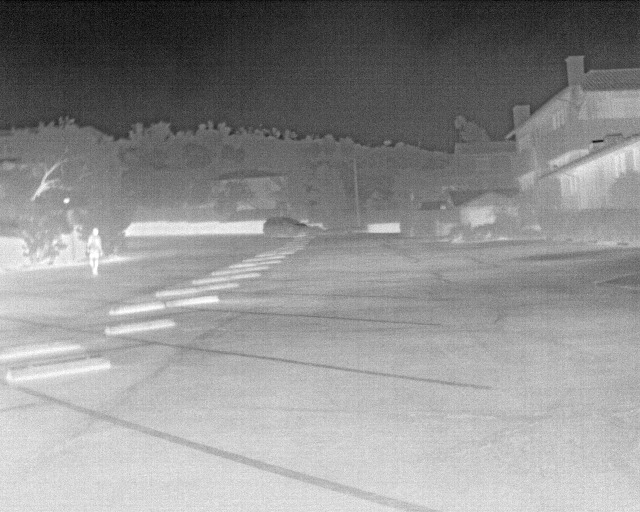
\includegraphics[width=\linewidth,height=0.4\textheight]{poster_video.jpg} % Usa una captura del vídeo
			}
			\vspace{0.1cm}
			\footnotesize \textcolor{gray}{\faYoutubePlay \hspace{0.1cm} Haz clic para reproducir vídeo externo}
		\end{block}
		
		\begin{itemize}
			\item \textbf{Verde:} Etiquetas reales (GT).
			\item \textbf{Rojo:} Detecciones del modelo.
		\end{itemize}
		
		% --- COLUMNA DERECHA: MÉTRICAS ---
		\column{0.35\textwidth}
		\begin{exampleblock}{Rendimiento en Test}
			\centering
			\vspace{0.2cm}
			{\Large \textbf{4.3 FPS}} \\
			\scriptsize Procesamiento por segundo
			\vspace{0.3cm}
			\hrule
			\vspace{0.3cm}
			{\Large \textbf{232.19}} \\
			\scriptsize ms / imagen
			\vspace{0.2cm}
		\end{exampleblock}
		
		\vspace{0.3cm}
		
		\begin{alertblock}{Hardware Local}
			\scriptsize
			\centering
			\textbf{CPU:} Intel Core i7-10510U \\
			\textbf{RAM:} 8 GB DDR4 \\
			\textbf{GPU:} Intel UHD Graphics \\
			\vspace{0.1cm}
			\textit{Inferencia en CPU}
		\end{alertblock}
	\end{columns}
	
	\end{frame}
	
	\begin{frame}{Rendimiento Global del Modelo}
		\begin{itemize}
			\item \textbf{Métricas globales:} Evolución de la precisión, recall, IOU y F1-score en función del umbral de confianza.
			\item \textbf{Bondad del clasificador:} Se obtiene un \textbf{MAP}\(=0.475\). 
		\end{itemize}
		
		\vfill
		
		\begin{figure}
			\centering
			% Ajustamos el ancho al 0.8 para que se vea grande pero deje aire
			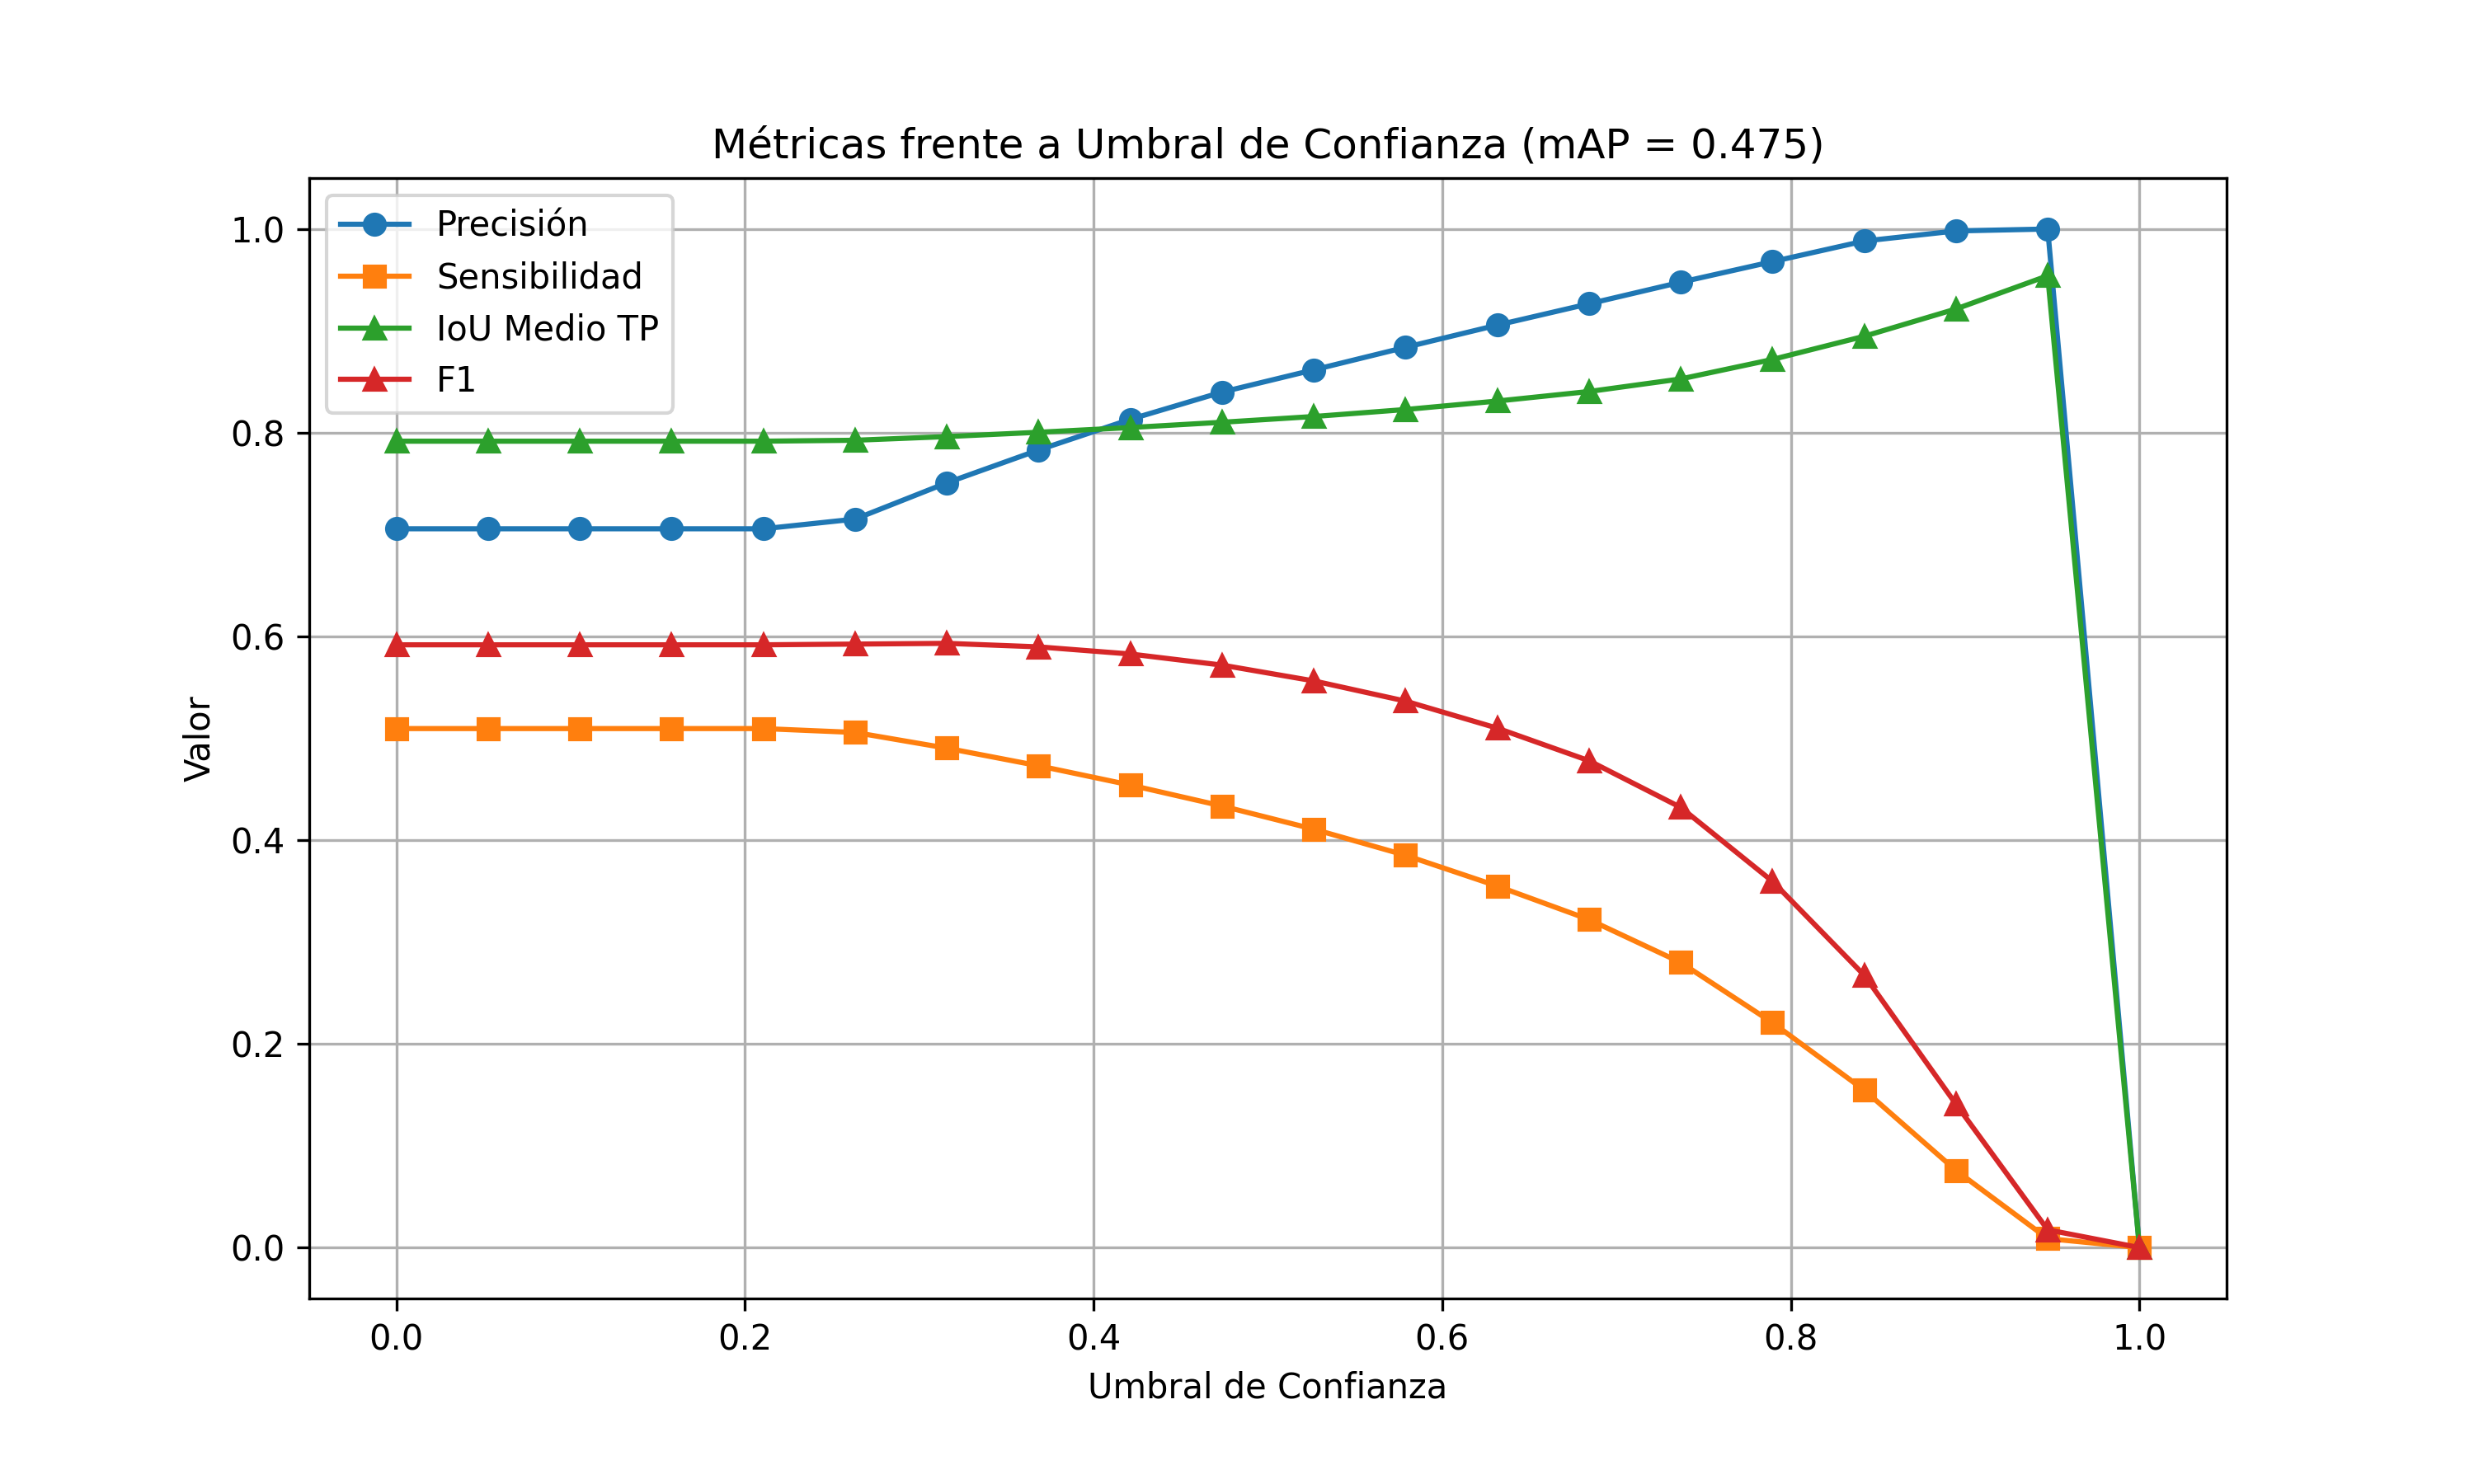
\includegraphics[width=0.6\linewidth, keepaspectratio]{metrics_vs_confidence}
			\caption{\small Curvas de métricas frente a la confianza para el conjunto de test.}
		\end{figure}
		
		\vfill
		
		\begin{center}
			\footnotesize \textit{Nota: El punto de cruce suele indicar el balance óptimo para el despliegue del modelo.}
		\end{center}
	\end{frame}
	
	\begin{frame}{Rendimiento Global del Modelo}
		\begin{itemize}
			\item \textbf{Métricas globales:} Evolución de la precisión, recall, IOU y F1-score en función del umbral de confianza.
			\item \textbf{Bondad del clasificador:} Se obtiene un \textbf{MAP}\(=0.475\). 
		\end{itemize}
		
		\vfill
		
		\begin{figure}
			\centering
			% Ajustamos el ancho al 0.8 para que se vea grande pero deje aire
			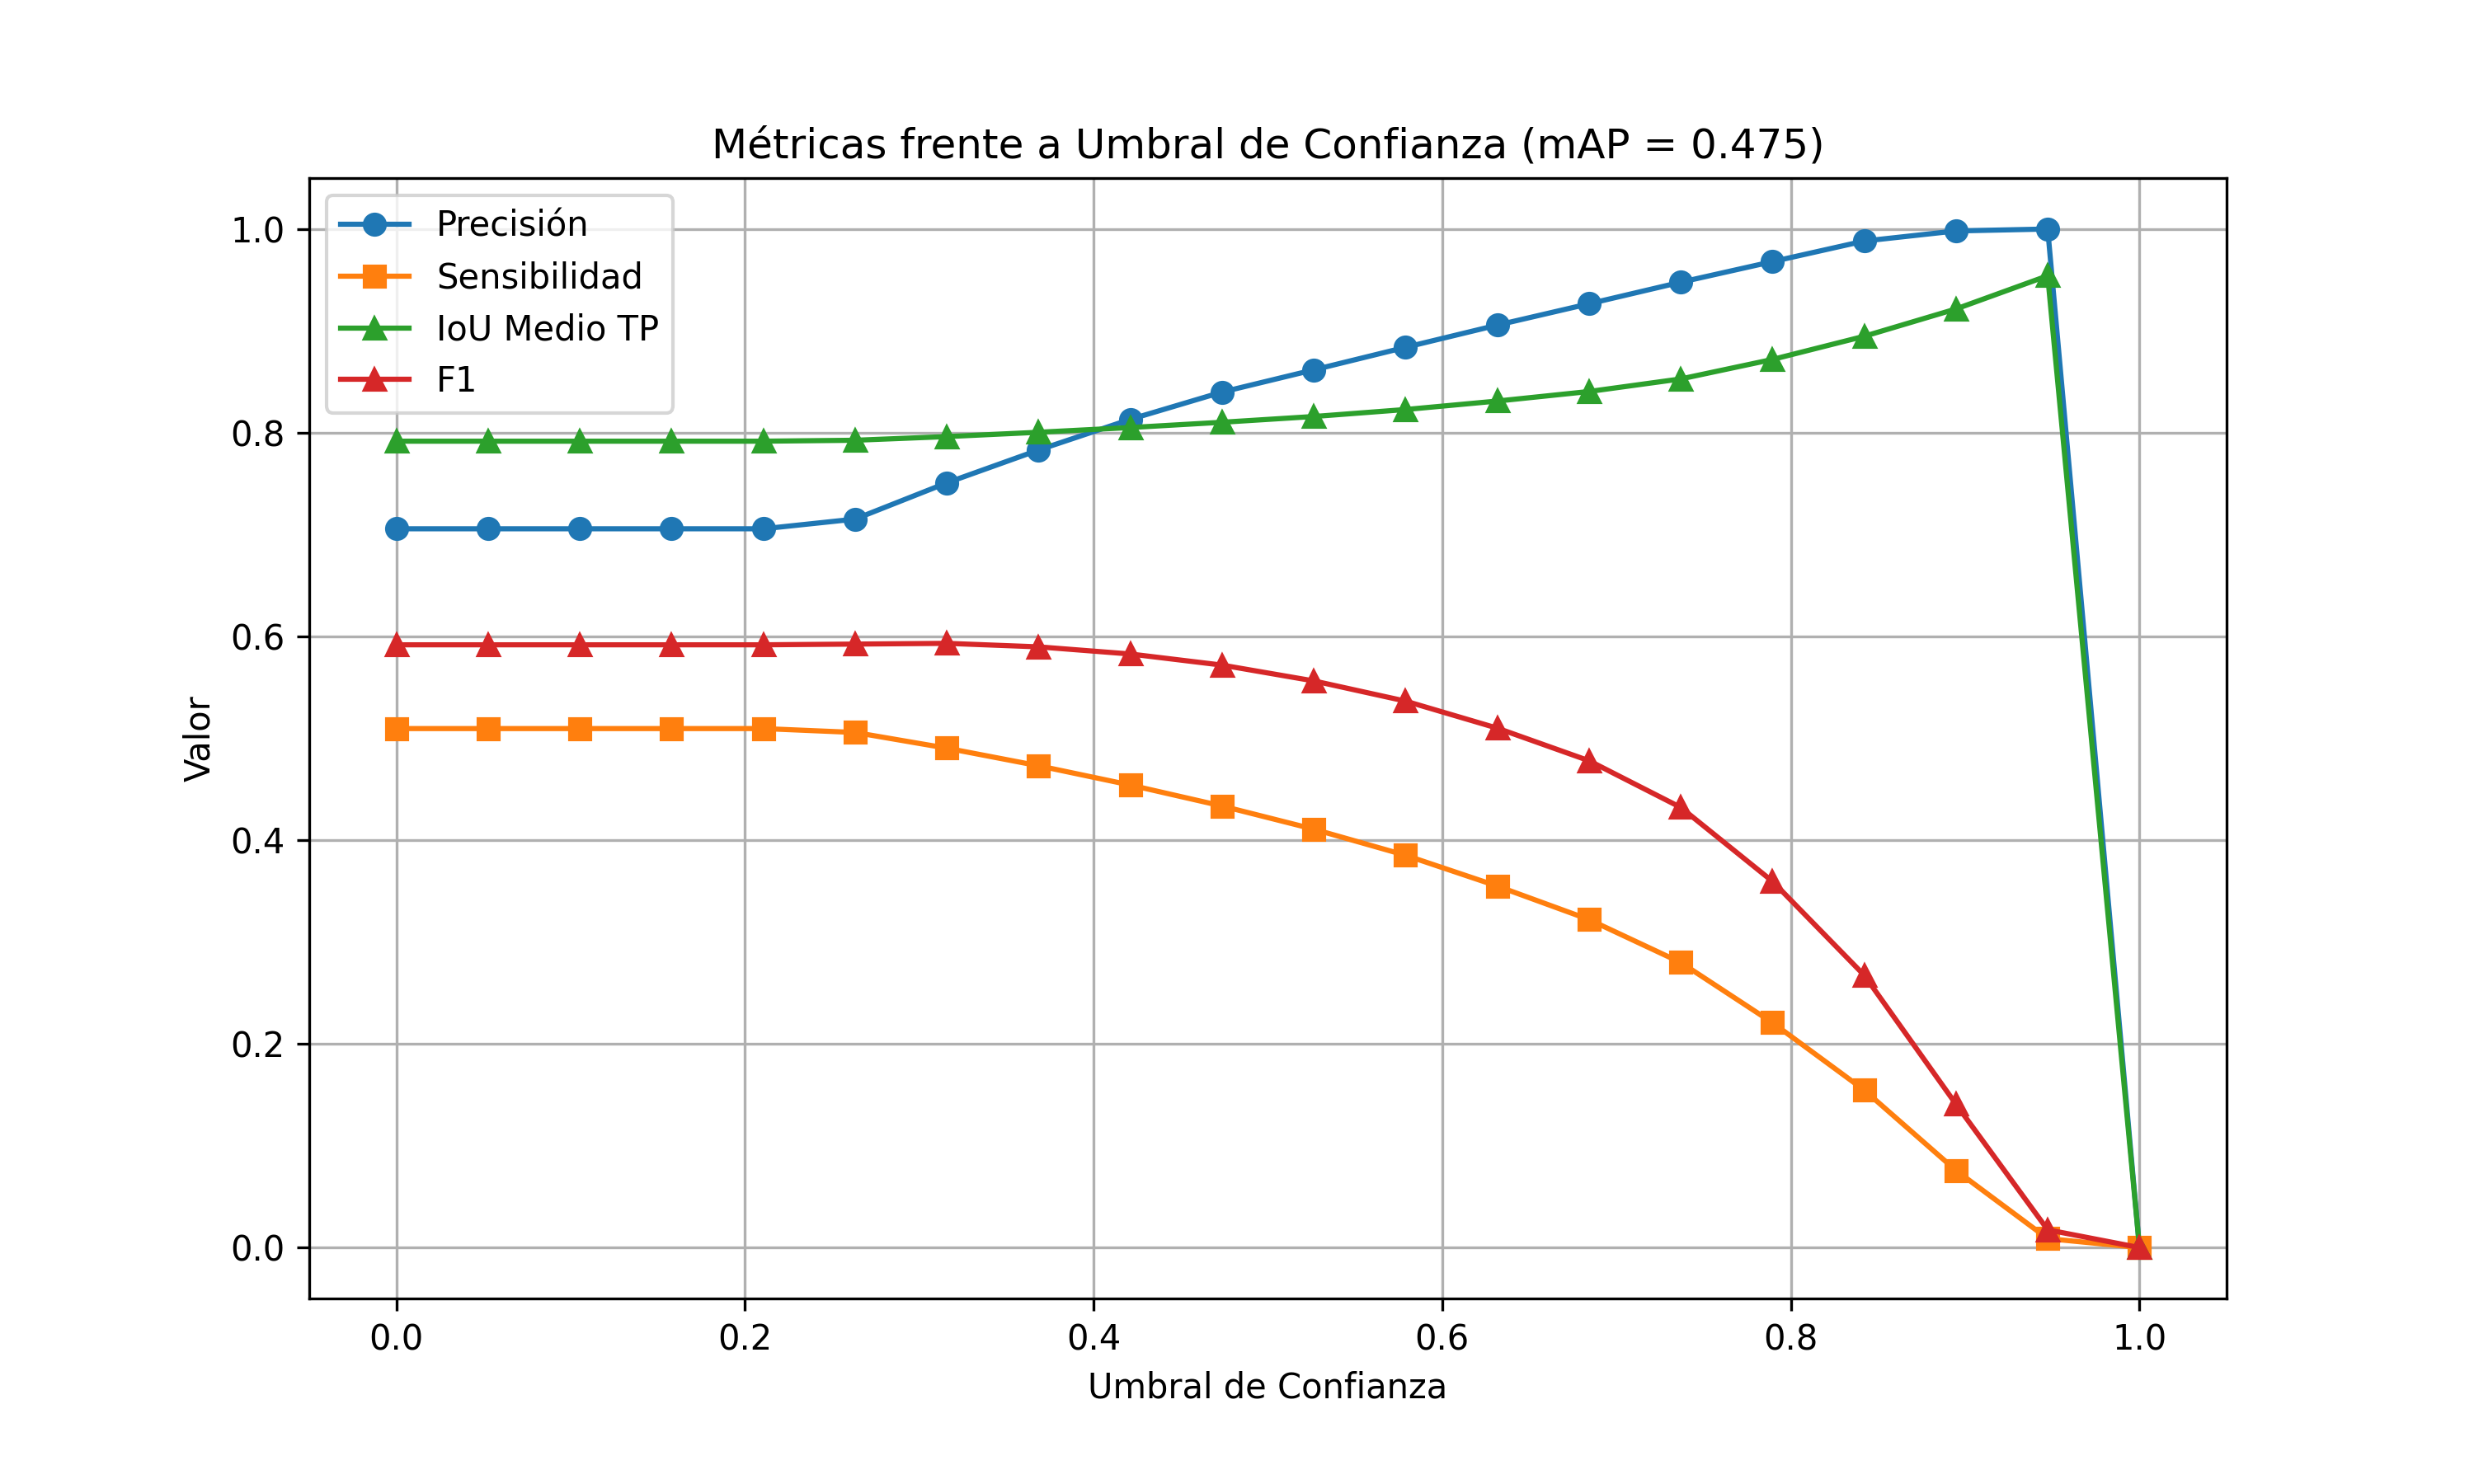
\includegraphics[width=0.6\linewidth, keepaspectratio]{metrics_vs_confidence}
			\caption{\small Curvas de métricas frente a la confianza para el conjunto de test.}
		\end{figure}
		
		\vfill
		
		\begin{center}
			\footnotesize \textit{Nota: El punto de cruce suele indicar el balance óptimo para el despliegue del modelo.}
		\end{center}
	\end{frame}
	\begin{frame}{Resultados Detallados por Categoría}
		\begin{figure}
			\centering
			\setlength{\tabcolsep}{2pt}
			\begin{tabular}{cc}
				\textbf{\scriptsize Persona} & \textbf{\scriptsize Coche} \\
				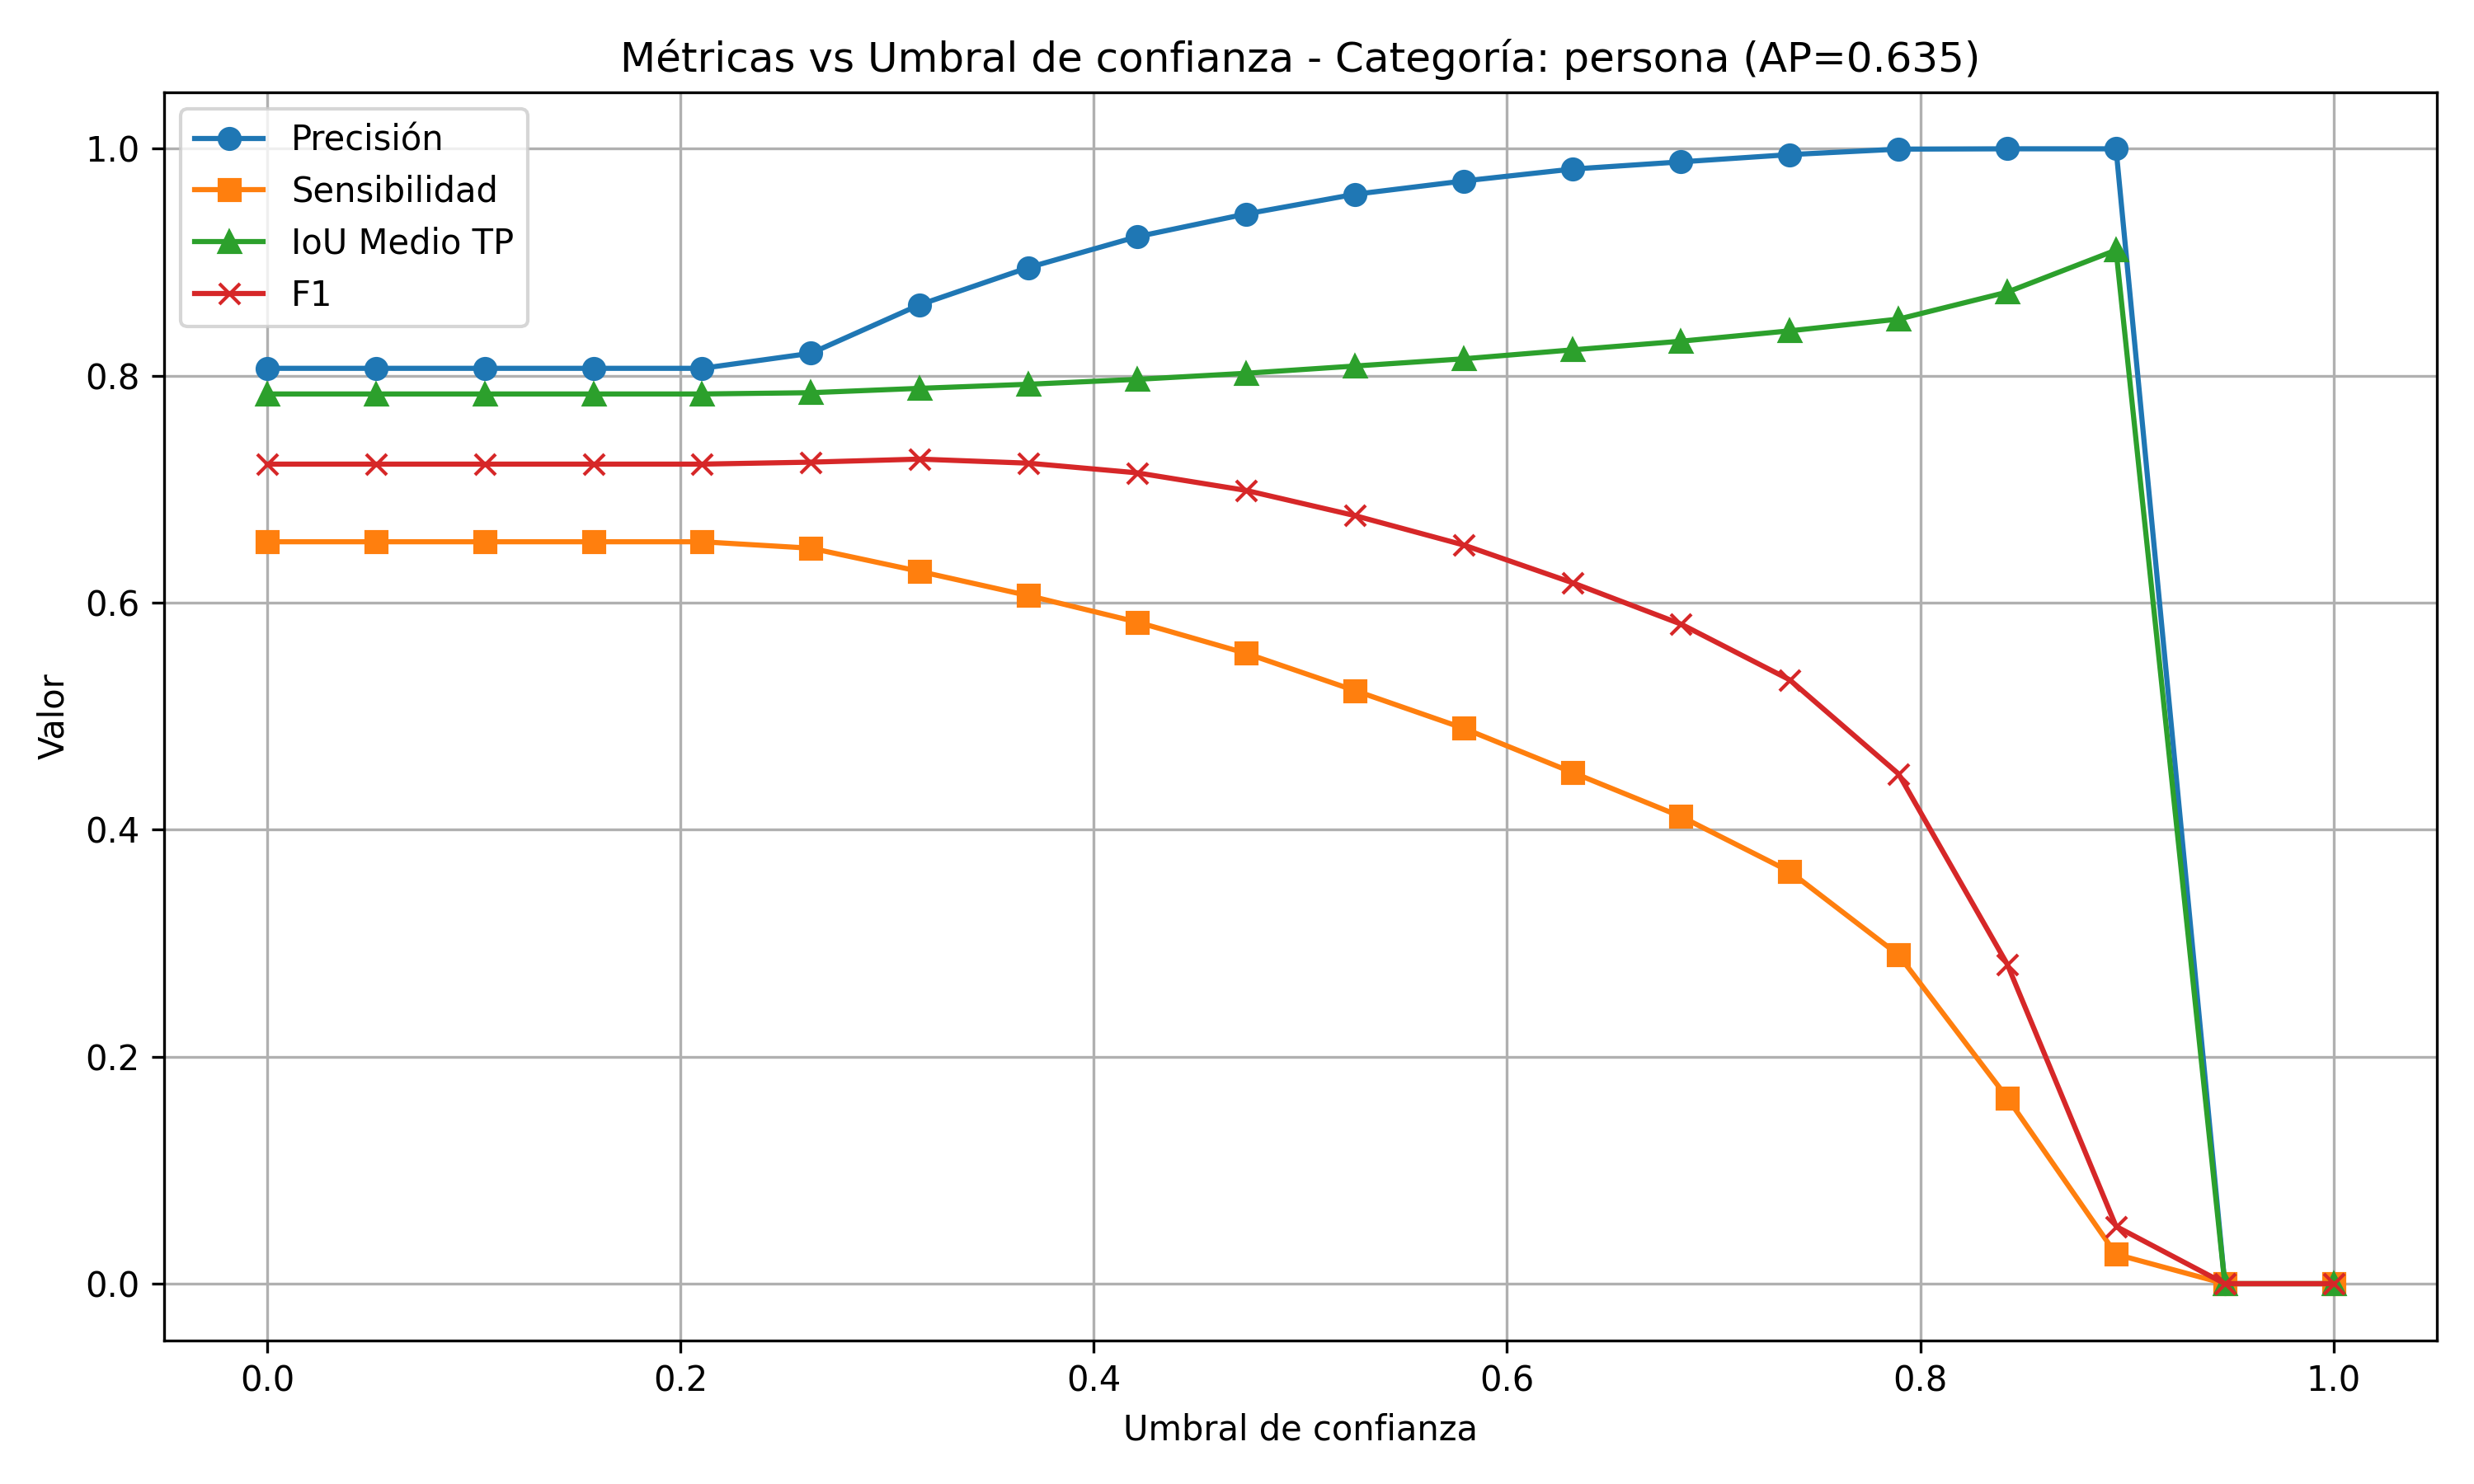
\includegraphics[height=2.8cm, width=4.5cm, keepaspectratio]{metrics_categoria_0.png} & 
				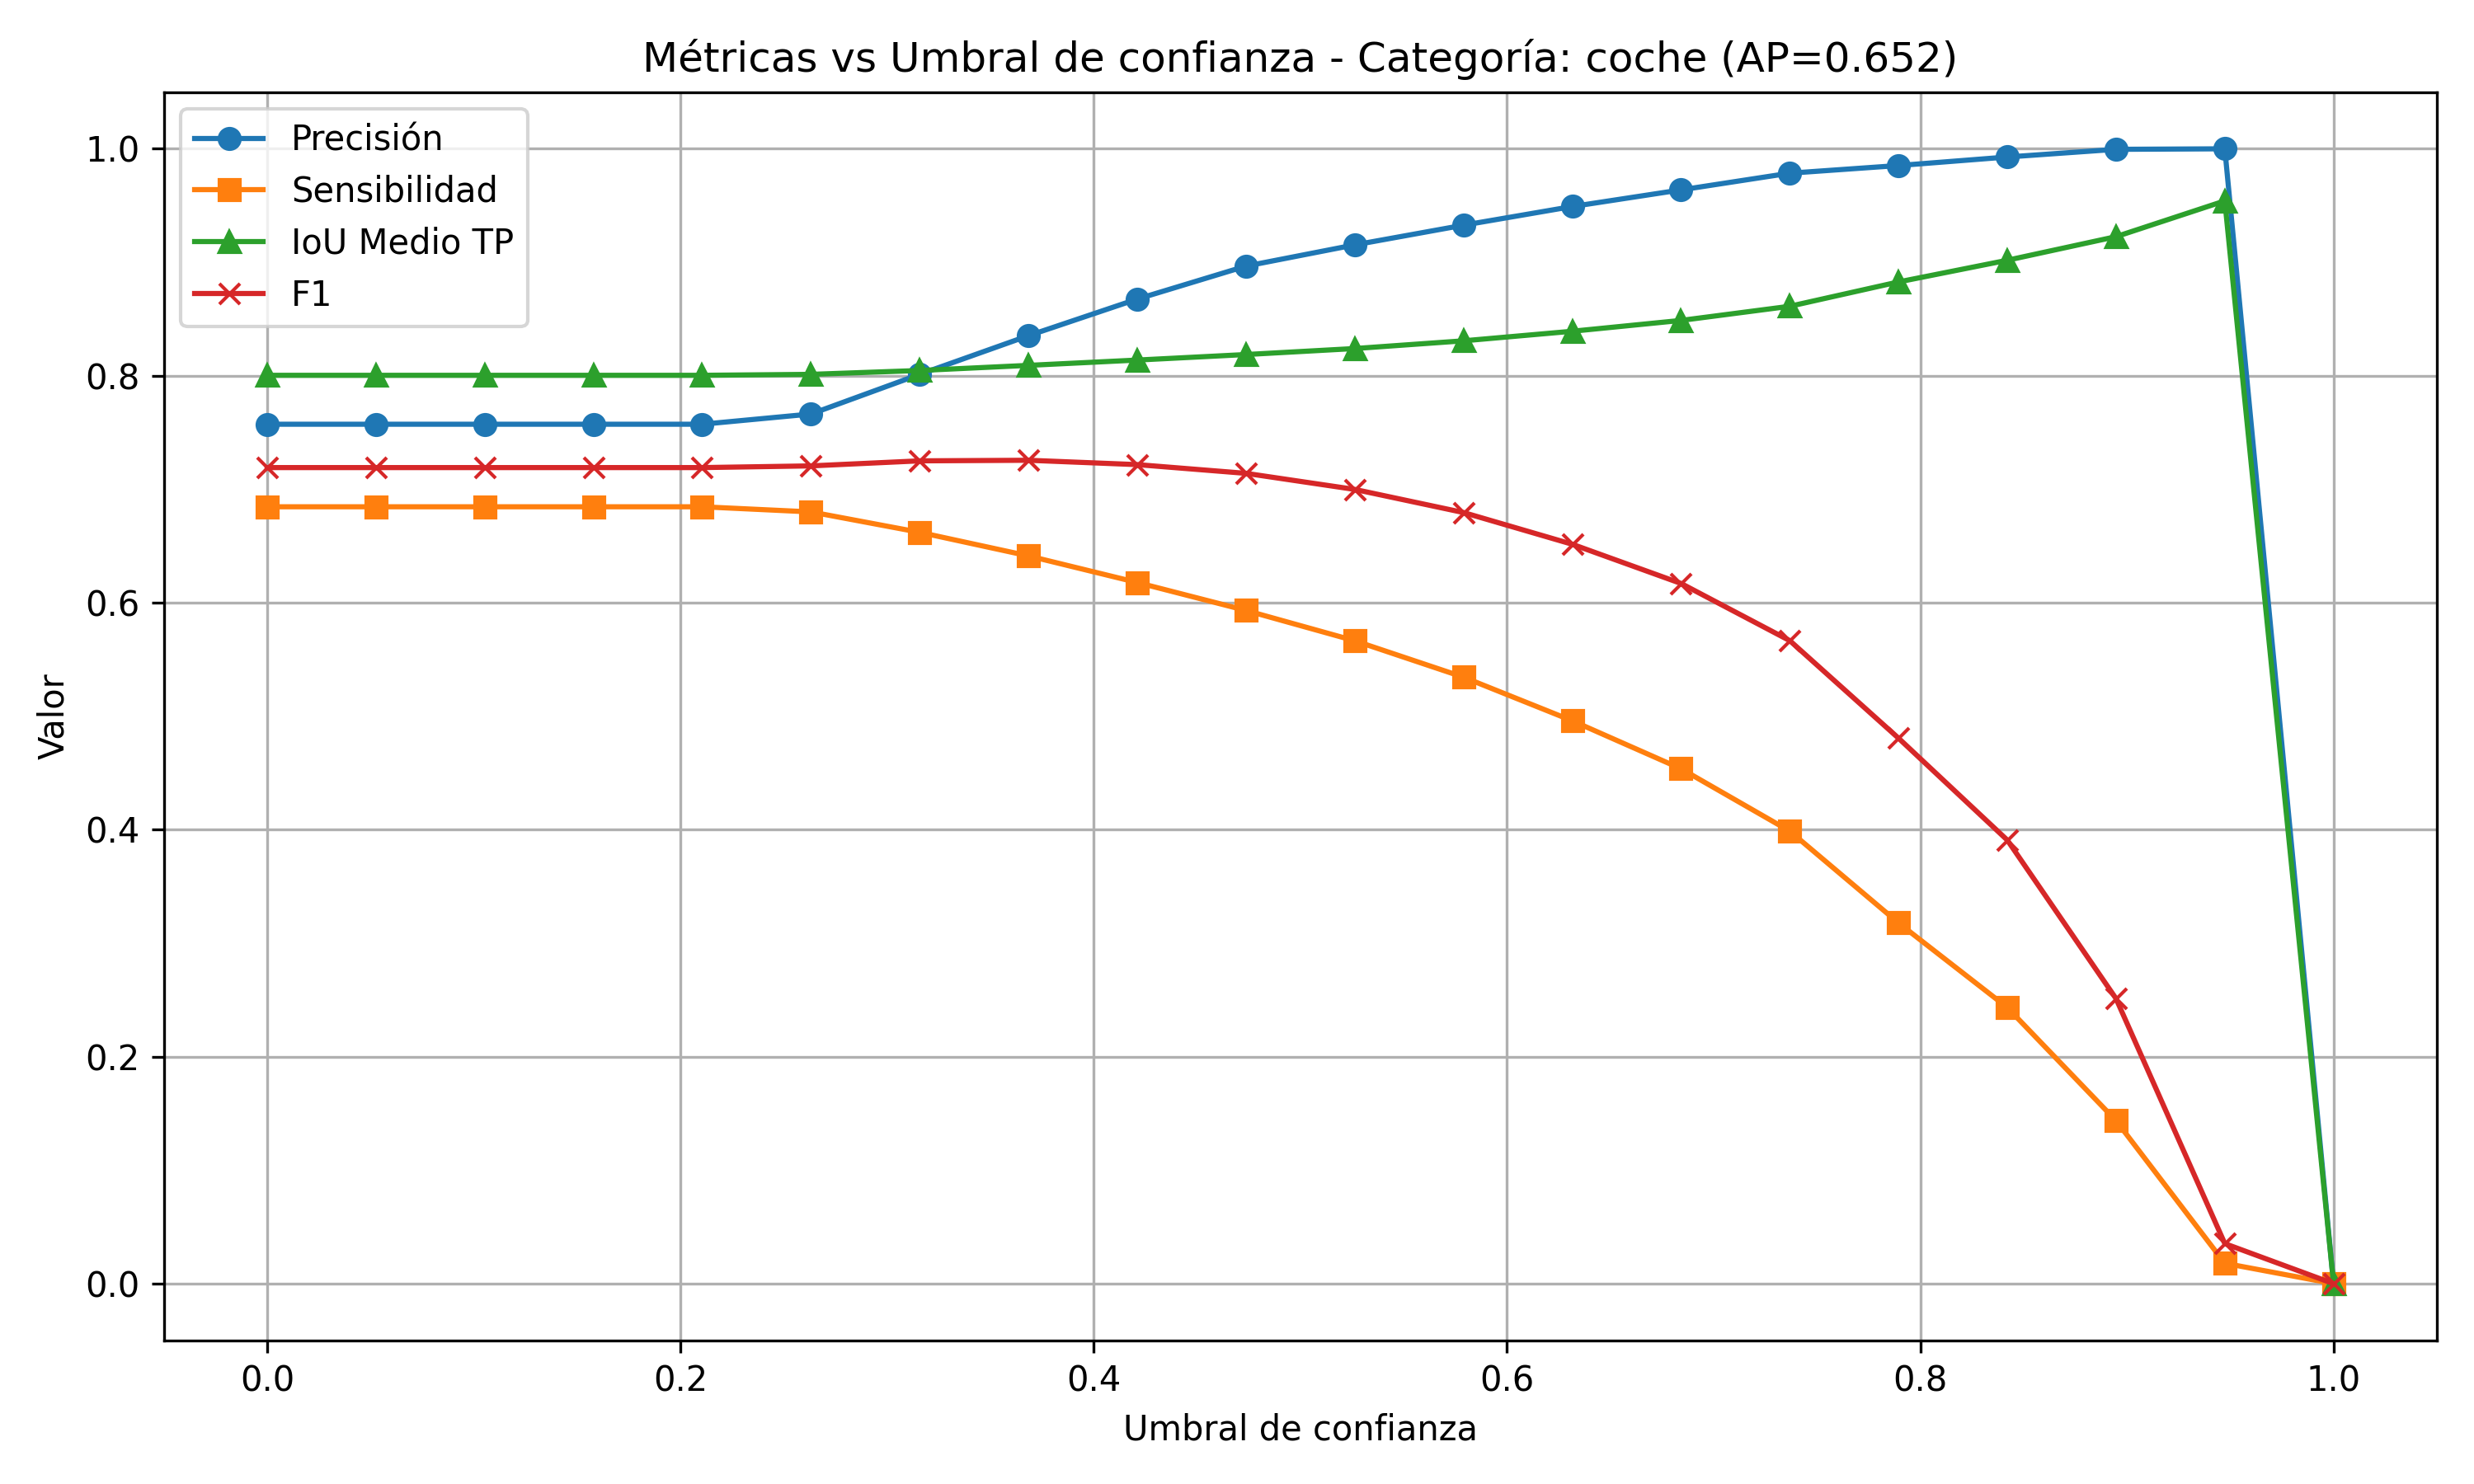
\includegraphics[height=2.8cm, width=4.5cm, keepaspectratio]{metrics_categoria_2.png} \\
				\\[-0.1cm]
				\textbf{\scriptsize Camión} & \textbf{\scriptsize Otros vehículos} \\
				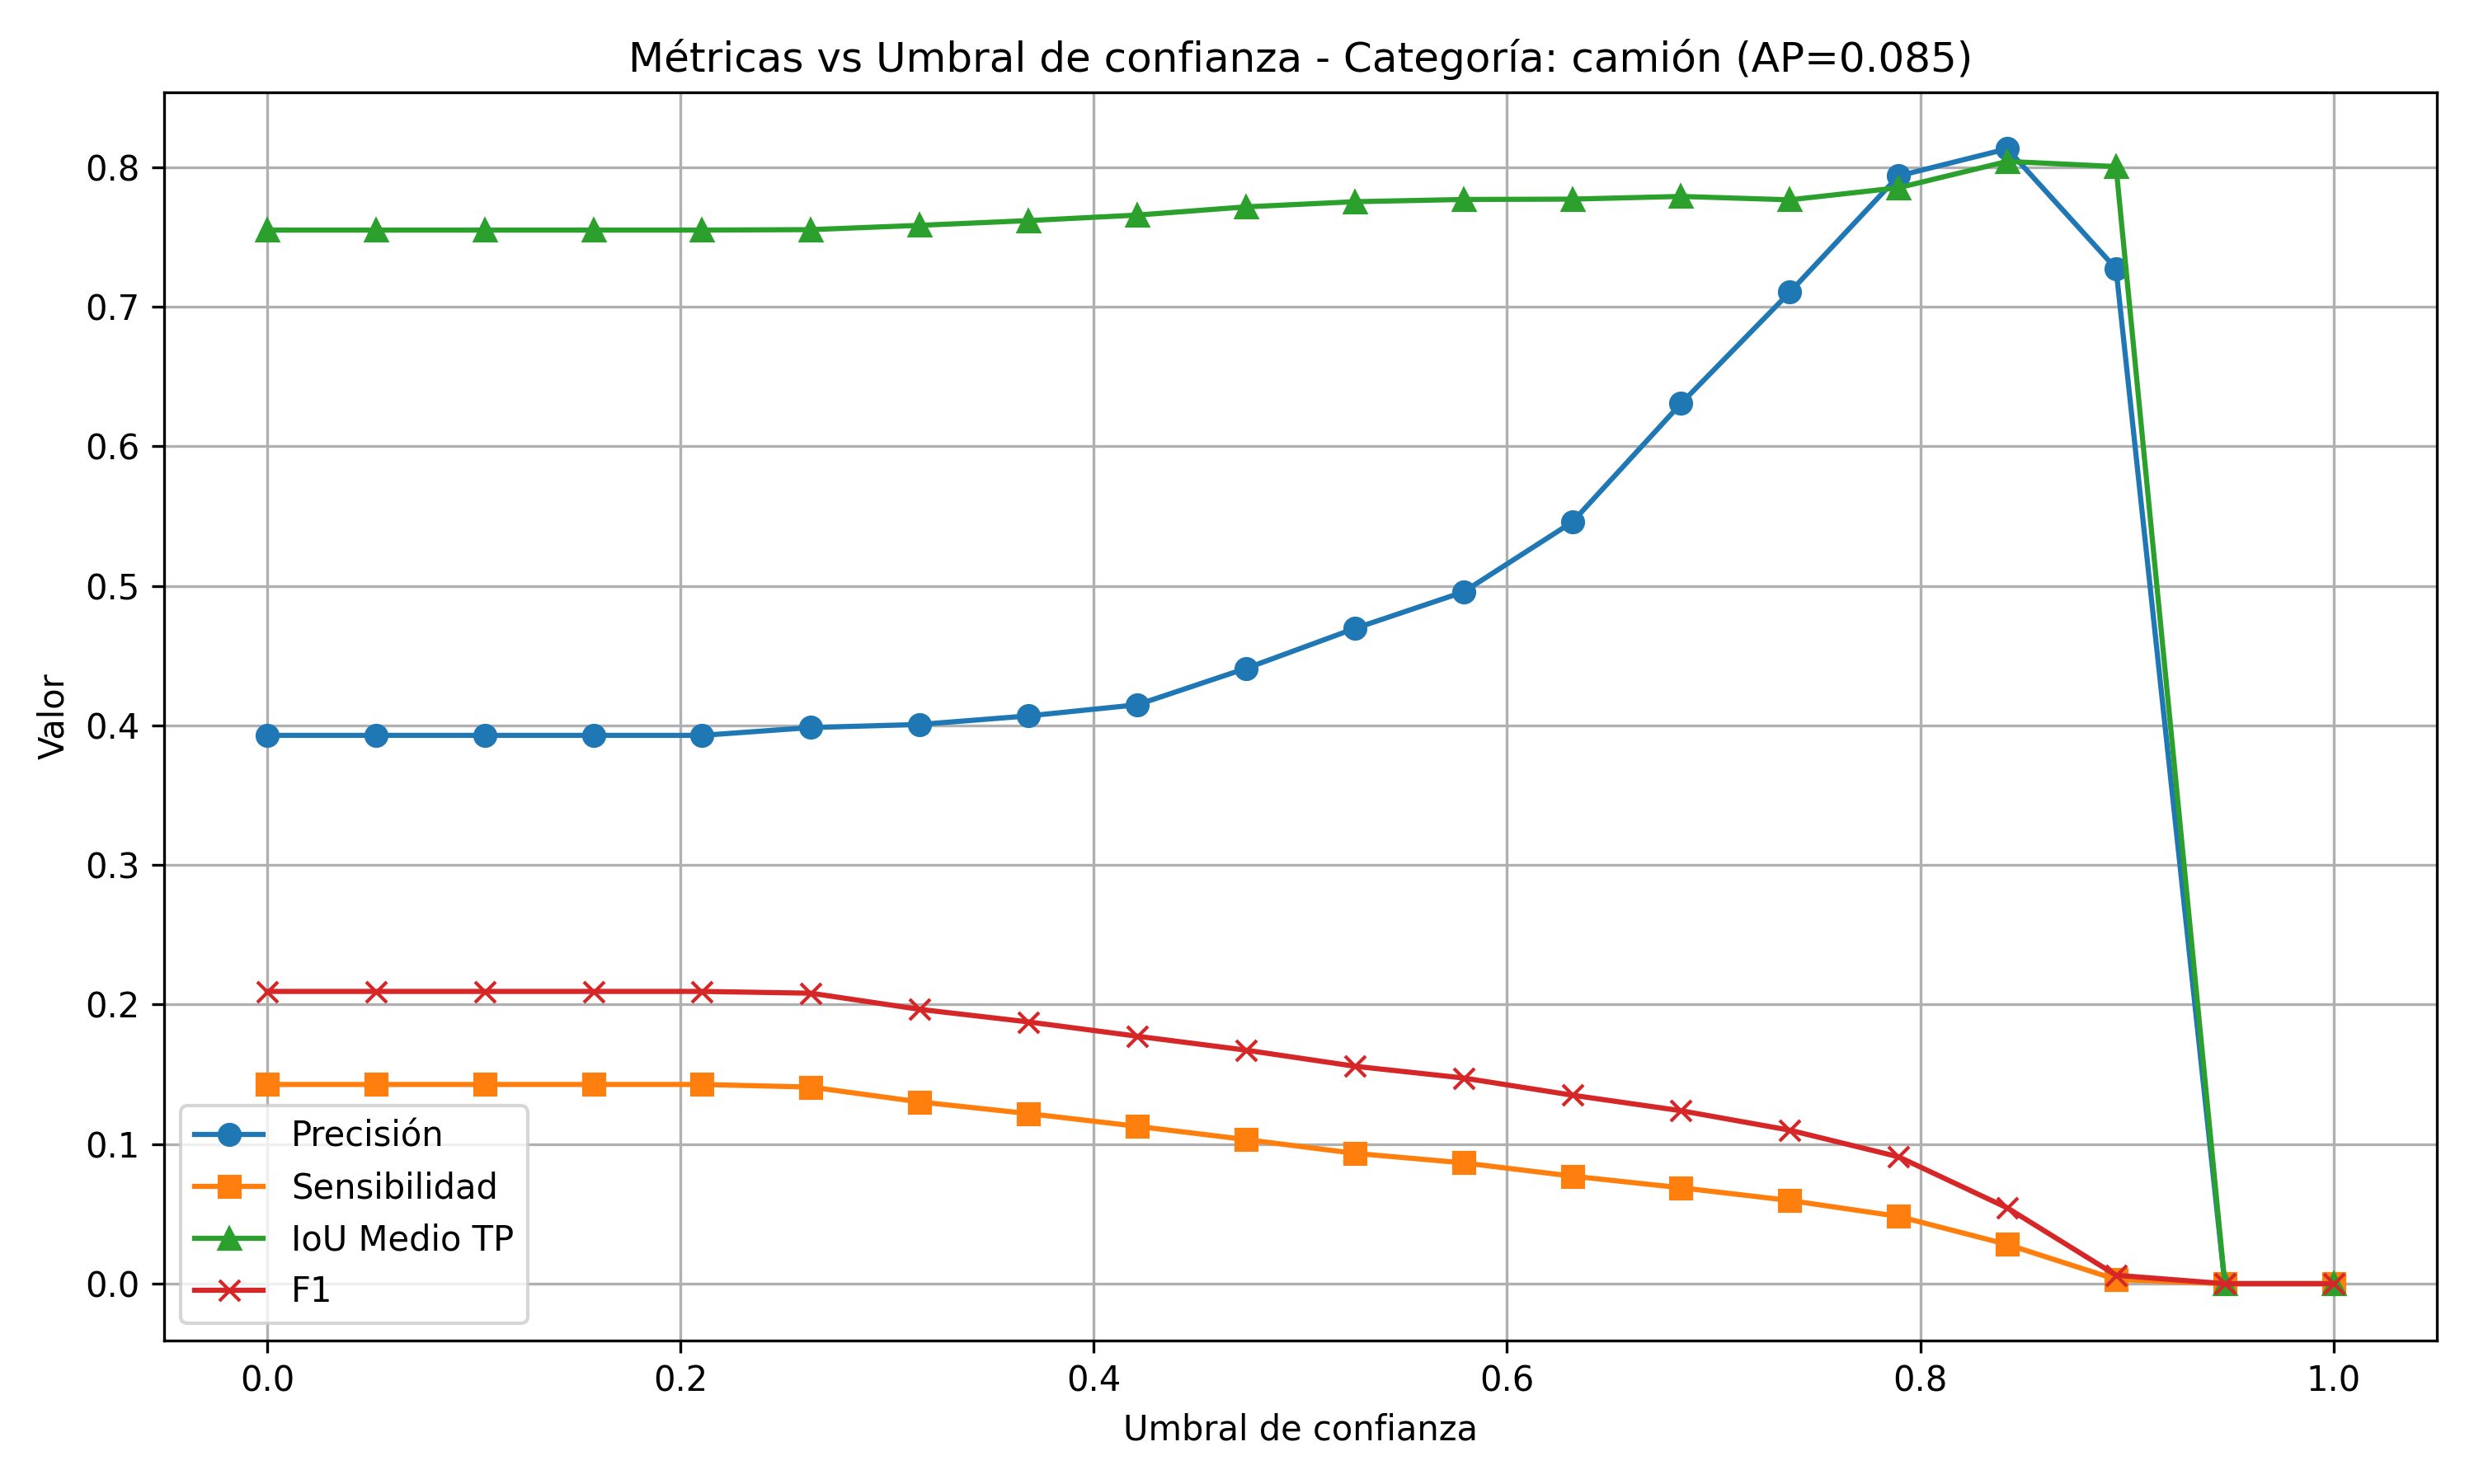
\includegraphics[height=2.8cm, width=4.5cm, keepaspectratio]{metrics_categoria_6.png} & 
				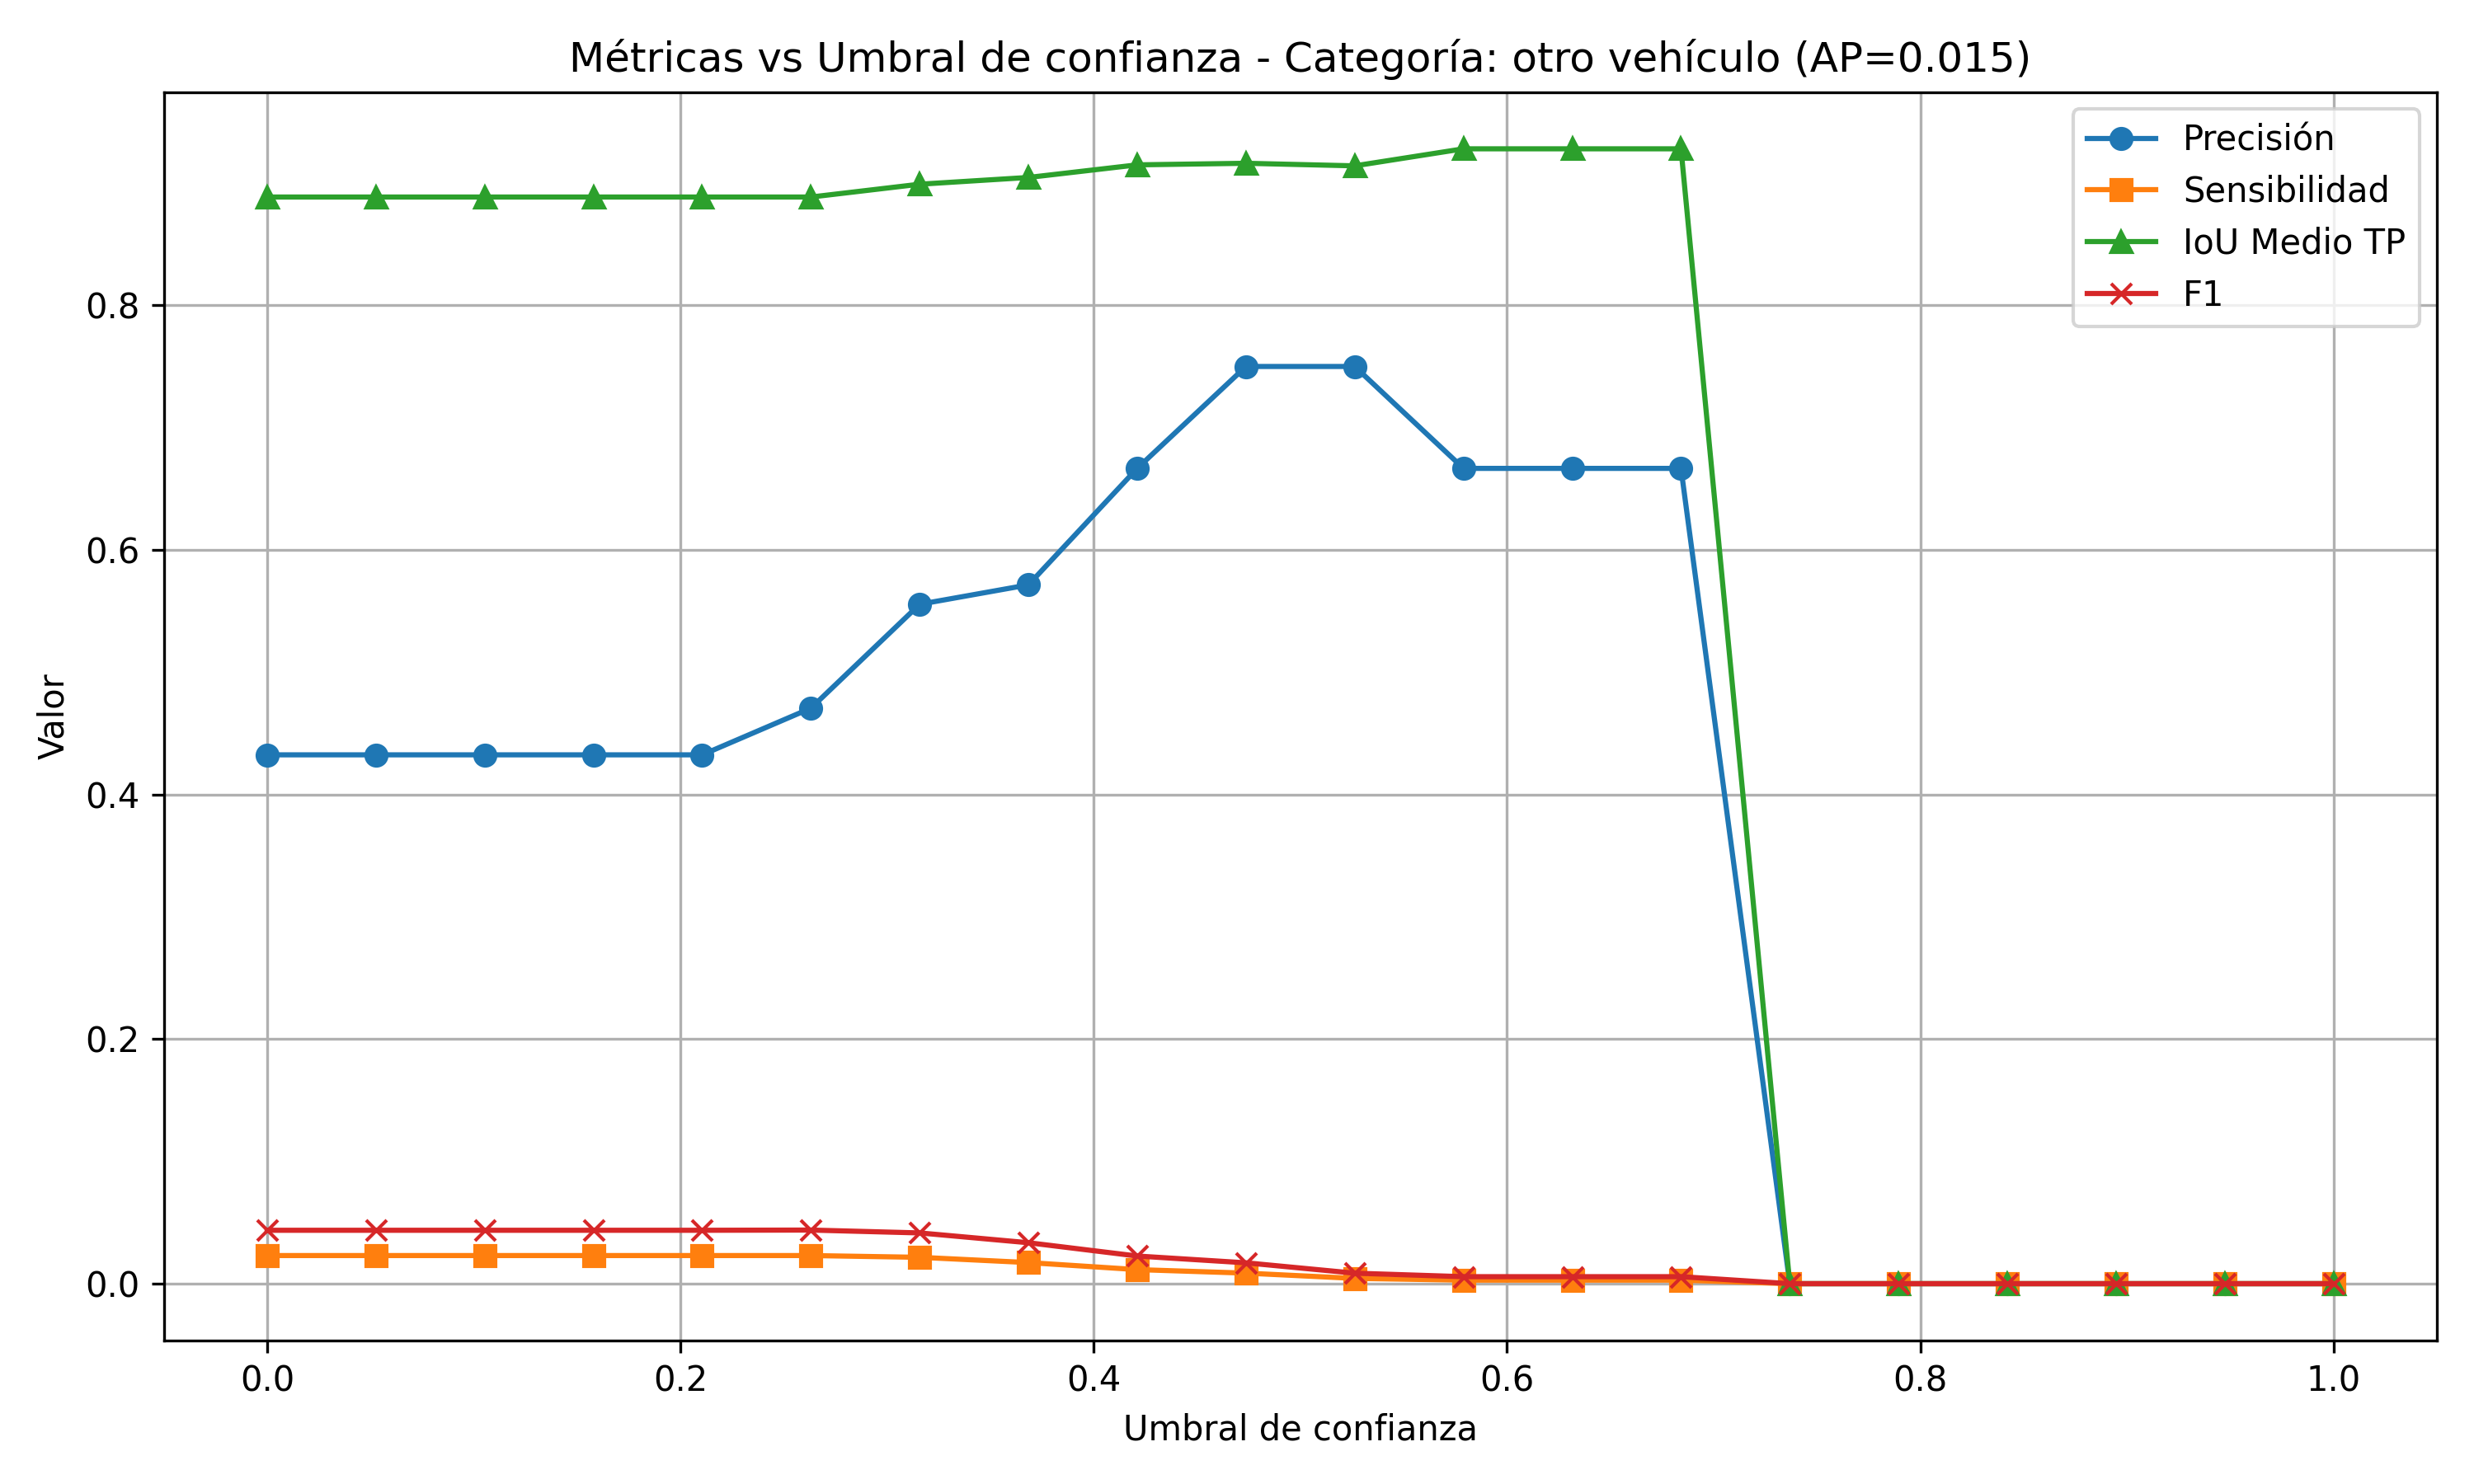
\includegraphics[height=2.8cm, width=4.5cm, keepaspectratio]{metrics_categoria_15.png}
			\end{tabular}
			\caption{\scriptsize Métricas del clasificador algunas categorías del conjunto de datos.}
		\end{figure}
	\end{frame}
	\begin{frame}{Curva Precisión-Recall (PR)}
		\begin{itemize}
			\item \textbf{Interpretación:} Evalúa el balance entre la exactitud de las detecciones y la capacidad del modelo para encontrar todos los objetos.
		\end{itemize}
		
		\vfill
		
		\begin{figure}
			\centering
			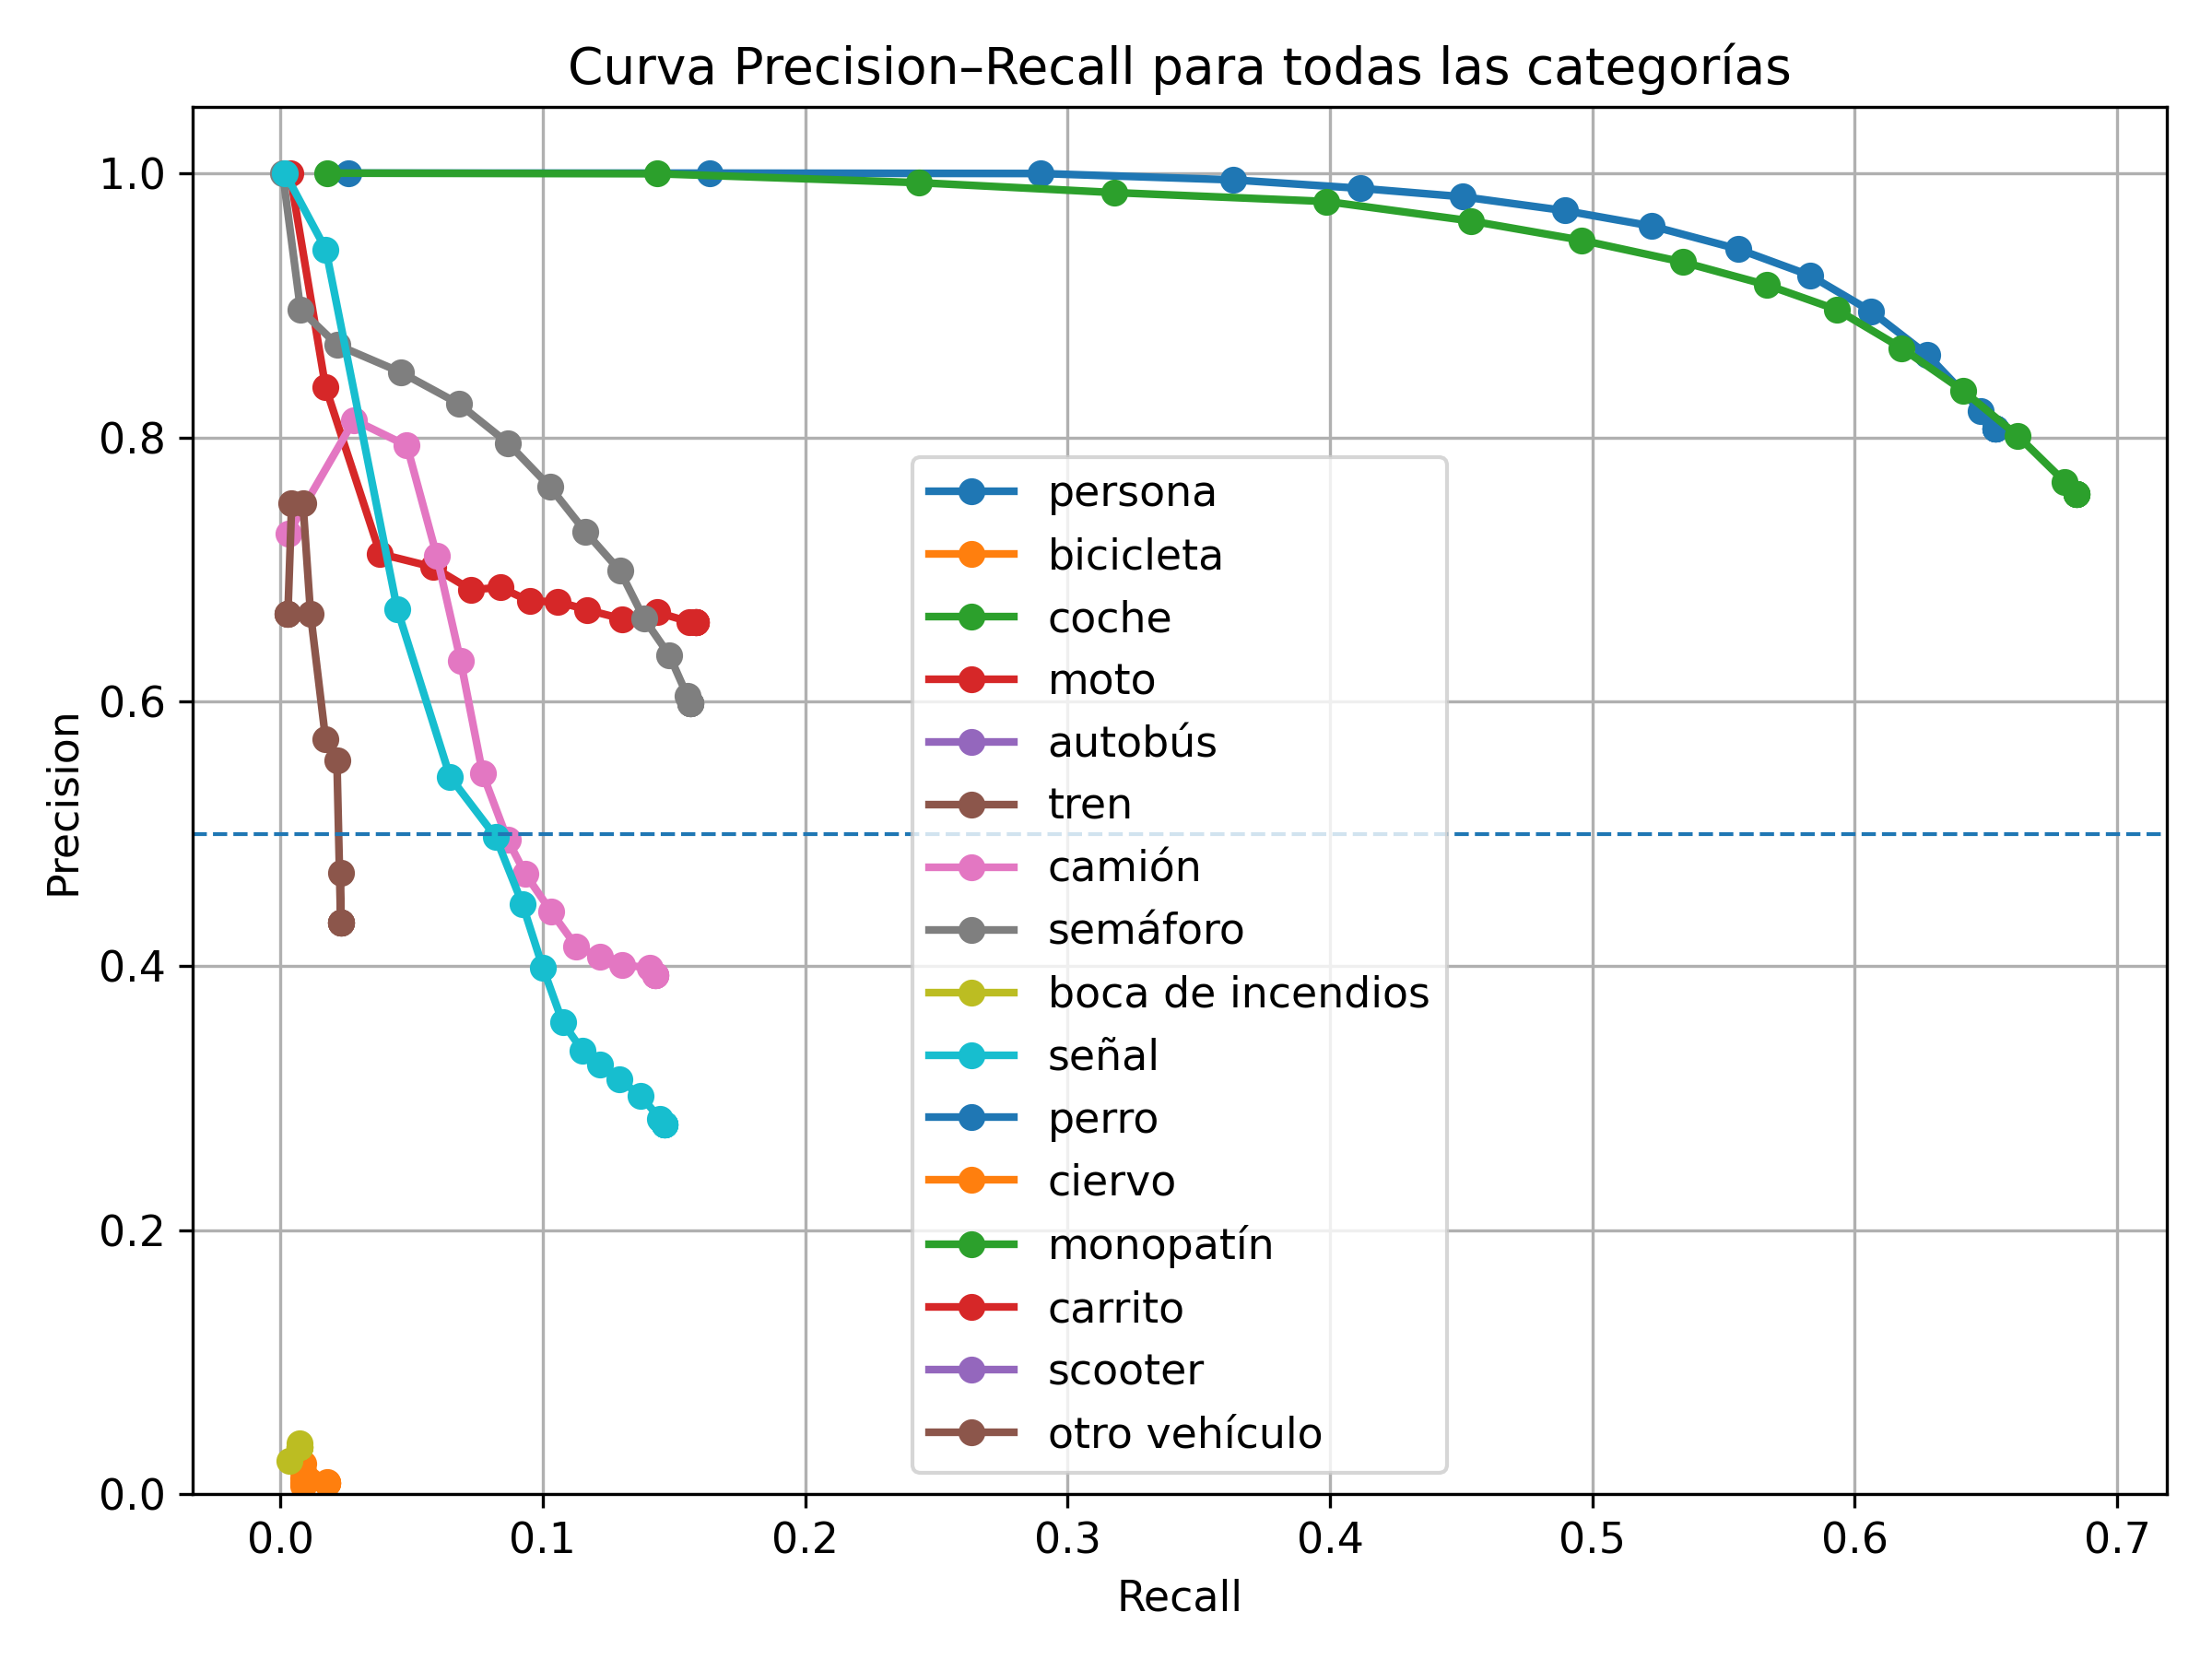
\includegraphics[width=0.5\linewidth, keepaspectratio]{precision-recall}
			\caption{\small Curva PR global: El modelo ideal tendería hacia la esquina superior derecha.}
		\end{figure}
		
		\vfill
		
		\begin{center}
			\footnotesize \textit{Nota: Una caída abrupta en la curva indicaría una pérdida de precisión al intentar aumentar la exhaustividad.}
		\end{center}
	\end{frame}
	
	\section{Conclusión}
		\begin{frame}{Índice}
		\tableofcontents[currentsection] 
	\end{frame}
		\begin{frame}{Resultados y Conclusión}
		\begin{block}{Implementación}
			\begin{itemize}
				\item \textbf{Entrada:} $640 \times 640$ monocanal (conversión 8-bits).
				\item \textbf{Dataset:} Teledyne FLIR (ADAS).
			\end{itemize}
		\end{block}
		
		\begin{alertblock}{Métricas Obtenidas}
			\begin{itemize}
				\item \textbf{mAP (Precisión Media):} 0.91 en peatones (oscuridad total).
				\item \textbf{Latencia:} 22ms por cuadro (Tiempo real).
			\end{itemize}
		\end{alertblock}
		
		\textbf{Conclusión:} YOLO + Sensores Térmicos es una solución robusta para vigilancia nocturna, superando limitaciones de cámaras RGB mediante análisis morfológico de firmas térmicas.
	\end{frame}
\end{document}